% generated by gen_launch_wave_fig.py -- do not edit by hand
\documentclass[10pt]{standalone}
\usepackage{helvet}
\renewcommand{\familydefault}{\sfdefault}
\usepackage{amsmath,amssymb}
\usepackage{tikz}
\usetikzlibrary{patterns}
\definecolor{csleep}{HTML}{D9D9D9}
\definecolor{cpark}{HTML}{F8CBAD}
\definecolor{cread}{HTML}{DDEBF7}
\definecolor{cwrite}{HTML}{FCE4D6}
\definecolor{cmiss}{HTML}{F4B6B6}
\definecolor{cjoin}{HTML}{FFE699}
\definecolor{chit}{HTML}{C6E0B4}
\definecolor{cld}{HTML}{C6E0B4}
\definecolor{cfpu}{HTML}{FFE699}
\definecolor{cspawn}{HTML}{D6E0EC}
\newcommand{\fs}{\fontsize{6.4}{7.4}\selectfont}
\newcommand{\fss}{\fontsize{5.6}{6.4}\selectfont}
\newcommand{\fv}{\fontsize{5.3}{5.8}\selectfont}
\begin{document}
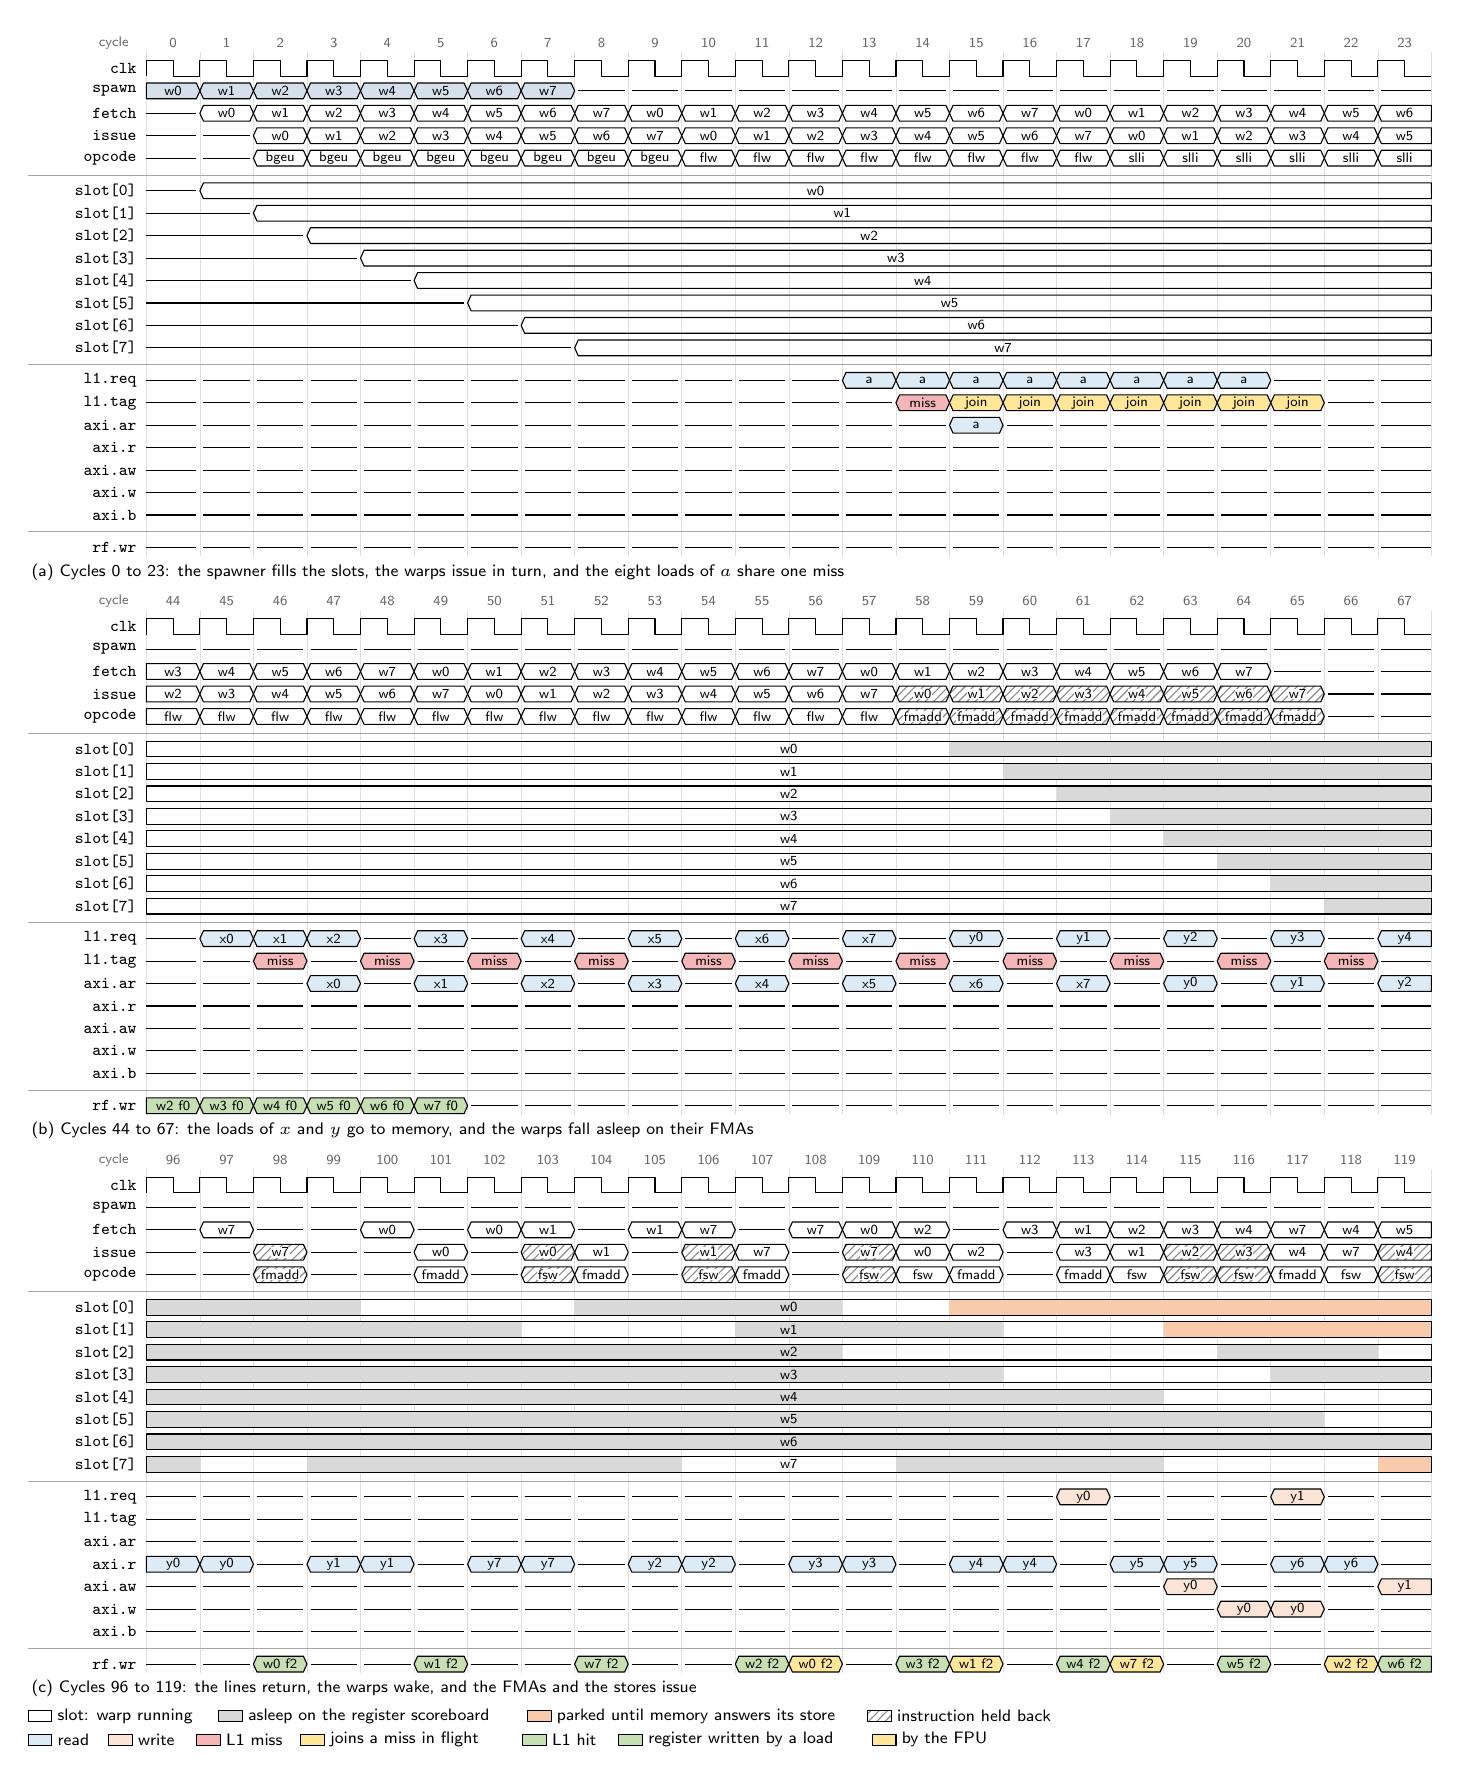
\begin{tikzpicture}[x=1cm, y=1cm,
  wire/.style={draw=black, line width=0.4pt, line join=round},
  gridline/.style={draw=black!12, line width=0.25pt},
  sep/.style={draw=black!35, line width=0.3pt},
  subcap/.style={font=\fs, inner sep=1pt},
  note/.style={font=\fss, inner sep=0.5pt, align=left}]

\node[font=\fv, text=black!60] at (1.890,-0.140) {0};
\node[font=\fv, text=black!60] at (2.570,-0.140) {1};
\node[font=\fv, text=black!60] at (3.250,-0.140) {2};
\node[font=\fv, text=black!60] at (3.930,-0.140) {3};
\node[font=\fv, text=black!60] at (4.610,-0.140) {4};
\node[font=\fv, text=black!60] at (5.290,-0.140) {5};
\node[font=\fv, text=black!60] at (5.970,-0.140) {6};
\node[font=\fv, text=black!60] at (6.650,-0.140) {7};
\node[font=\fv, text=black!60] at (7.330,-0.140) {8};
\node[font=\fv, text=black!60] at (8.010,-0.140) {9};
\node[font=\fv, text=black!60] at (8.690,-0.140) {10};
\node[font=\fv, text=black!60] at (9.370,-0.140) {11};
\node[font=\fv, text=black!60] at (10.050,-0.140) {12};
\node[font=\fv, text=black!60] at (10.730,-0.140) {13};
\node[font=\fv, text=black!60] at (11.410,-0.140) {14};
\node[font=\fv, text=black!60] at (12.090,-0.140) {15};
\node[font=\fv, text=black!60] at (12.770,-0.140) {16};
\node[font=\fv, text=black!60] at (13.450,-0.140) {17};
\node[font=\fv, text=black!60] at (14.130,-0.140) {18};
\node[font=\fv, text=black!60] at (14.810,-0.140) {19};
\node[font=\fv, text=black!60] at (15.490,-0.140) {20};
\node[font=\fv, text=black!60] at (16.170,-0.140) {21};
\node[font=\fv, text=black!60] at (16.850,-0.140) {22};
\node[font=\fv, text=black!60] at (17.530,-0.140) {23};
\draw[gridline] (1.550,-0.260) -- (1.550,-6.660);
\draw[gridline] (2.230,-0.260) -- (2.230,-6.660);
\draw[gridline] (2.910,-0.260) -- (2.910,-6.660);
\draw[gridline] (3.590,-0.260) -- (3.590,-6.660);
\draw[gridline] (4.270,-0.260) -- (4.270,-6.660);
\draw[gridline] (4.950,-0.260) -- (4.950,-6.660);
\draw[gridline] (5.630,-0.260) -- (5.630,-6.660);
\draw[gridline] (6.310,-0.260) -- (6.310,-6.660);
\draw[gridline] (6.990,-0.260) -- (6.990,-6.660);
\draw[gridline] (7.670,-0.260) -- (7.670,-6.660);
\draw[gridline] (8.350,-0.260) -- (8.350,-6.660);
\draw[gridline] (9.030,-0.260) -- (9.030,-6.660);
\draw[gridline] (9.710,-0.260) -- (9.710,-6.660);
\draw[gridline] (10.390,-0.260) -- (10.390,-6.660);
\draw[gridline] (11.070,-0.260) -- (11.070,-6.660);
\draw[gridline] (11.750,-0.260) -- (11.750,-6.660);
\draw[gridline] (12.430,-0.260) -- (12.430,-6.660);
\draw[gridline] (13.110,-0.260) -- (13.110,-6.660);
\draw[gridline] (13.790,-0.260) -- (13.790,-6.660);
\draw[gridline] (14.470,-0.260) -- (14.470,-6.660);
\draw[gridline] (15.150,-0.260) -- (15.150,-6.660);
\draw[gridline] (15.830,-0.260) -- (15.830,-6.660);
\draw[gridline] (16.510,-0.260) -- (16.510,-6.660);
\draw[gridline] (17.190,-0.260) -- (17.190,-6.660);
\draw[gridline] (17.870,-0.260) -- (17.870,-6.660);
\node[anchor=east, font=\fv, text=black!60] at (1.450,-0.140) {cycle};
\node[anchor=east, font=\fss\ttfamily, inner sep=0.5pt] at (1.450,-0.463) {clk};
\draw[wire] (1.550,-0.562) -- (1.550,-0.362) -- (1.890,-0.362) -- (1.890,-0.562) -- (2.230,-0.562) -- (2.230,-0.362) -- (2.570,-0.362) -- (2.570,-0.562) -- (2.910,-0.562) -- (2.910,-0.362) -- (3.250,-0.362) -- (3.250,-0.562) -- (3.590,-0.562) -- (3.590,-0.362) -- (3.930,-0.362) -- (3.930,-0.562) -- (4.270,-0.562) -- (4.270,-0.362) -- (4.610,-0.362) -- (4.610,-0.562) -- (4.950,-0.562) -- (4.950,-0.362) -- (5.290,-0.362) -- (5.290,-0.562) -- (5.630,-0.562) -- (5.630,-0.362) -- (5.970,-0.362) -- (5.970,-0.562) -- (6.310,-0.562) -- (6.310,-0.362) -- (6.650,-0.362) -- (6.650,-0.562) -- (6.990,-0.562) -- (6.990,-0.362) -- (7.330,-0.362) -- (7.330,-0.562) -- (7.670,-0.562) -- (7.670,-0.362) -- (8.010,-0.362) -- (8.010,-0.562) -- (8.350,-0.562) -- (8.350,-0.362) -- (8.690,-0.362) -- (8.690,-0.562) -- (9.030,-0.562) -- (9.030,-0.362) -- (9.370,-0.362) -- (9.370,-0.562) -- (9.710,-0.562) -- (9.710,-0.362) -- (10.050,-0.362) -- (10.050,-0.562) -- (10.390,-0.562) -- (10.390,-0.362) -- (10.730,-0.362) -- (10.730,-0.562) -- (11.070,-0.562) -- (11.070,-0.362) -- (11.410,-0.362) -- (11.410,-0.562) -- (11.750,-0.562) -- (11.750,-0.362) -- (12.090,-0.362) -- (12.090,-0.562) -- (12.430,-0.562) -- (12.430,-0.362) -- (12.770,-0.362) -- (12.770,-0.562) -- (13.110,-0.562) -- (13.110,-0.362) -- (13.450,-0.362) -- (13.450,-0.562) -- (13.790,-0.562) -- (13.790,-0.362) -- (14.130,-0.362) -- (14.130,-0.562) -- (14.470,-0.562) -- (14.470,-0.362) -- (14.810,-0.362) -- (14.810,-0.562) -- (15.150,-0.562) -- (15.150,-0.362) -- (15.490,-0.362) -- (15.490,-0.562) -- (15.830,-0.562) -- (15.830,-0.362) -- (16.170,-0.362) -- (16.170,-0.562) -- (16.510,-0.562) -- (16.510,-0.362) -- (16.850,-0.362) -- (16.850,-0.562) -- (17.190,-0.562) -- (17.190,-0.362) -- (17.530,-0.362) -- (17.530,-0.562) -- (17.870,-0.562);
\node[anchor=east, font=\fss\ttfamily, inner sep=0.5pt] at (1.450,-0.747) {spawn};
\draw[wire, fill=cspawn] (1.550,-0.647) -- (2.185,-0.647) -- (2.230,-0.747) -- (2.185,-0.847) -- (1.550,-0.847) -- (1.550,-0.747) -- cycle;
\node[font=\fv, inner sep=0pt] at (1.890,-0.747) {w0};
\draw[wire, fill=cspawn] (2.275,-0.647) -- (2.865,-0.647) -- (2.910,-0.747) -- (2.865,-0.847) -- (2.275,-0.847) -- (2.230,-0.747) -- cycle;
\node[font=\fv, inner sep=0pt] at (2.570,-0.747) {w1};
\draw[wire, fill=cspawn] (2.955,-0.647) -- (3.545,-0.647) -- (3.590,-0.747) -- (3.545,-0.847) -- (2.955,-0.847) -- (2.910,-0.747) -- cycle;
\node[font=\fv, inner sep=0pt] at (3.250,-0.747) {w2};
\draw[wire, fill=cspawn] (3.635,-0.647) -- (4.225,-0.647) -- (4.270,-0.747) -- (4.225,-0.847) -- (3.635,-0.847) -- (3.590,-0.747) -- cycle;
\node[font=\fv, inner sep=0pt] at (3.930,-0.747) {w3};
\draw[wire, fill=cspawn] (4.315,-0.647) -- (4.905,-0.647) -- (4.950,-0.747) -- (4.905,-0.847) -- (4.315,-0.847) -- (4.270,-0.747) -- cycle;
\node[font=\fv, inner sep=0pt] at (4.610,-0.747) {w4};
\draw[wire, fill=cspawn] (4.995,-0.647) -- (5.585,-0.647) -- (5.630,-0.747) -- (5.585,-0.847) -- (4.995,-0.847) -- (4.950,-0.747) -- cycle;
\node[font=\fv, inner sep=0pt] at (5.290,-0.747) {w5};
\draw[wire, fill=cspawn] (5.675,-0.647) -- (6.265,-0.647) -- (6.310,-0.747) -- (6.265,-0.847) -- (5.675,-0.847) -- (5.630,-0.747) -- cycle;
\node[font=\fv, inner sep=0pt] at (5.970,-0.747) {w6};
\draw[wire, fill=cspawn] (6.355,-0.647) -- (6.945,-0.647) -- (6.990,-0.747) -- (6.945,-0.847) -- (6.355,-0.847) -- (6.310,-0.747) -- cycle;
\node[font=\fv, inner sep=0pt] at (6.650,-0.747) {w7};
\draw[wire] (7.035,-0.747) -- (7.625,-0.747);
\draw[wire] (7.715,-0.747) -- (8.305,-0.747);
\draw[wire] (8.395,-0.747) -- (8.985,-0.747);
\draw[wire] (9.075,-0.747) -- (9.665,-0.747);
\draw[wire] (9.755,-0.747) -- (10.345,-0.747);
\draw[wire] (10.435,-0.747) -- (11.025,-0.747);
\draw[wire] (11.115,-0.747) -- (11.705,-0.747);
\draw[wire] (11.795,-0.747) -- (12.385,-0.747);
\draw[wire] (12.475,-0.747) -- (13.065,-0.747);
\draw[wire] (13.155,-0.747) -- (13.745,-0.747);
\draw[wire] (13.835,-0.747) -- (14.425,-0.747);
\draw[wire] (14.515,-0.747) -- (15.105,-0.747);
\draw[wire] (15.195,-0.747) -- (15.785,-0.747);
\draw[wire] (15.875,-0.747) -- (16.465,-0.747);
\draw[wire] (16.555,-0.747) -- (17.145,-0.747);
\draw[wire] (17.235,-0.747) -- (17.870,-0.747);
\node[anchor=east, font=\fss\ttfamily, inner sep=0.5pt] at (1.450,-1.032) {fetch};
\draw[wire] (1.550,-1.032) -- (2.185,-1.032);
\draw[wire, fill=white] (2.275,-0.932) -- (2.865,-0.932) -- (2.910,-1.032) -- (2.865,-1.132) -- (2.275,-1.132) -- (2.230,-1.032) -- cycle;
\node[font=\fv, inner sep=0pt] at (2.570,-1.032) {w0};
\draw[wire, fill=white] (2.955,-0.932) -- (3.545,-0.932) -- (3.590,-1.032) -- (3.545,-1.132) -- (2.955,-1.132) -- (2.910,-1.032) -- cycle;
\node[font=\fv, inner sep=0pt] at (3.250,-1.032) {w1};
\draw[wire, fill=white] (3.635,-0.932) -- (4.225,-0.932) -- (4.270,-1.032) -- (4.225,-1.132) -- (3.635,-1.132) -- (3.590,-1.032) -- cycle;
\node[font=\fv, inner sep=0pt] at (3.930,-1.032) {w2};
\draw[wire, fill=white] (4.315,-0.932) -- (4.905,-0.932) -- (4.950,-1.032) -- (4.905,-1.132) -- (4.315,-1.132) -- (4.270,-1.032) -- cycle;
\node[font=\fv, inner sep=0pt] at (4.610,-1.032) {w3};
\draw[wire, fill=white] (4.995,-0.932) -- (5.585,-0.932) -- (5.630,-1.032) -- (5.585,-1.132) -- (4.995,-1.132) -- (4.950,-1.032) -- cycle;
\node[font=\fv, inner sep=0pt] at (5.290,-1.032) {w4};
\draw[wire, fill=white] (5.675,-0.932) -- (6.265,-0.932) -- (6.310,-1.032) -- (6.265,-1.132) -- (5.675,-1.132) -- (5.630,-1.032) -- cycle;
\node[font=\fv, inner sep=0pt] at (5.970,-1.032) {w5};
\draw[wire, fill=white] (6.355,-0.932) -- (6.945,-0.932) -- (6.990,-1.032) -- (6.945,-1.132) -- (6.355,-1.132) -- (6.310,-1.032) -- cycle;
\node[font=\fv, inner sep=0pt] at (6.650,-1.032) {w6};
\draw[wire, fill=white] (7.035,-0.932) -- (7.625,-0.932) -- (7.670,-1.032) -- (7.625,-1.132) -- (7.035,-1.132) -- (6.990,-1.032) -- cycle;
\node[font=\fv, inner sep=0pt] at (7.330,-1.032) {w7};
\draw[wire, fill=white] (7.715,-0.932) -- (8.305,-0.932) -- (8.350,-1.032) -- (8.305,-1.132) -- (7.715,-1.132) -- (7.670,-1.032) -- cycle;
\node[font=\fv, inner sep=0pt] at (8.010,-1.032) {w0};
\draw[wire, fill=white] (8.395,-0.932) -- (8.985,-0.932) -- (9.030,-1.032) -- (8.985,-1.132) -- (8.395,-1.132) -- (8.350,-1.032) -- cycle;
\node[font=\fv, inner sep=0pt] at (8.690,-1.032) {w1};
\draw[wire, fill=white] (9.075,-0.932) -- (9.665,-0.932) -- (9.710,-1.032) -- (9.665,-1.132) -- (9.075,-1.132) -- (9.030,-1.032) -- cycle;
\node[font=\fv, inner sep=0pt] at (9.370,-1.032) {w2};
\draw[wire, fill=white] (9.755,-0.932) -- (10.345,-0.932) -- (10.390,-1.032) -- (10.345,-1.132) -- (9.755,-1.132) -- (9.710,-1.032) -- cycle;
\node[font=\fv, inner sep=0pt] at (10.050,-1.032) {w3};
\draw[wire, fill=white] (10.435,-0.932) -- (11.025,-0.932) -- (11.070,-1.032) -- (11.025,-1.132) -- (10.435,-1.132) -- (10.390,-1.032) -- cycle;
\node[font=\fv, inner sep=0pt] at (10.730,-1.032) {w4};
\draw[wire, fill=white] (11.115,-0.932) -- (11.705,-0.932) -- (11.750,-1.032) -- (11.705,-1.132) -- (11.115,-1.132) -- (11.070,-1.032) -- cycle;
\node[font=\fv, inner sep=0pt] at (11.410,-1.032) {w5};
\draw[wire, fill=white] (11.795,-0.932) -- (12.385,-0.932) -- (12.430,-1.032) -- (12.385,-1.132) -- (11.795,-1.132) -- (11.750,-1.032) -- cycle;
\node[font=\fv, inner sep=0pt] at (12.090,-1.032) {w6};
\draw[wire, fill=white] (12.475,-0.932) -- (13.065,-0.932) -- (13.110,-1.032) -- (13.065,-1.132) -- (12.475,-1.132) -- (12.430,-1.032) -- cycle;
\node[font=\fv, inner sep=0pt] at (12.770,-1.032) {w7};
\draw[wire, fill=white] (13.155,-0.932) -- (13.745,-0.932) -- (13.790,-1.032) -- (13.745,-1.132) -- (13.155,-1.132) -- (13.110,-1.032) -- cycle;
\node[font=\fv, inner sep=0pt] at (13.450,-1.032) {w0};
\draw[wire, fill=white] (13.835,-0.932) -- (14.425,-0.932) -- (14.470,-1.032) -- (14.425,-1.132) -- (13.835,-1.132) -- (13.790,-1.032) -- cycle;
\node[font=\fv, inner sep=0pt] at (14.130,-1.032) {w1};
\draw[wire, fill=white] (14.515,-0.932) -- (15.105,-0.932) -- (15.150,-1.032) -- (15.105,-1.132) -- (14.515,-1.132) -- (14.470,-1.032) -- cycle;
\node[font=\fv, inner sep=0pt] at (14.810,-1.032) {w2};
\draw[wire, fill=white] (15.195,-0.932) -- (15.785,-0.932) -- (15.830,-1.032) -- (15.785,-1.132) -- (15.195,-1.132) -- (15.150,-1.032) -- cycle;
\node[font=\fv, inner sep=0pt] at (15.490,-1.032) {w3};
\draw[wire, fill=white] (15.875,-0.932) -- (16.465,-0.932) -- (16.510,-1.032) -- (16.465,-1.132) -- (15.875,-1.132) -- (15.830,-1.032) -- cycle;
\node[font=\fv, inner sep=0pt] at (16.170,-1.032) {w4};
\draw[wire, fill=white] (16.555,-0.932) -- (17.145,-0.932) -- (17.190,-1.032) -- (17.145,-1.132) -- (16.555,-1.132) -- (16.510,-1.032) -- cycle;
\node[font=\fv, inner sep=0pt] at (16.850,-1.032) {w5};
\draw[wire, fill=white] (17.235,-0.932) -- (17.870,-0.932) -- (17.870,-1.032) -- (17.870,-1.132) -- (17.235,-1.132) -- (17.190,-1.032) -- cycle;
\node[font=\fv, inner sep=0pt] at (17.530,-1.032) {w6};
\node[anchor=east, font=\fss\ttfamily, inner sep=0.5pt] at (1.450,-1.317) {issue};
\draw[wire] (1.550,-1.317) -- (2.185,-1.317);
\draw[wire] (2.275,-1.317) -- (2.865,-1.317);
\draw[wire, fill=white] (2.955,-1.217) -- (3.545,-1.217) -- (3.590,-1.317) -- (3.545,-1.417) -- (2.955,-1.417) -- (2.910,-1.317) -- cycle;
\node[font=\fv, inner sep=0pt] at (3.250,-1.317) {w0};
\draw[wire, fill=white] (3.635,-1.217) -- (4.225,-1.217) -- (4.270,-1.317) -- (4.225,-1.417) -- (3.635,-1.417) -- (3.590,-1.317) -- cycle;
\node[font=\fv, inner sep=0pt] at (3.930,-1.317) {w1};
\draw[wire, fill=white] (4.315,-1.217) -- (4.905,-1.217) -- (4.950,-1.317) -- (4.905,-1.417) -- (4.315,-1.417) -- (4.270,-1.317) -- cycle;
\node[font=\fv, inner sep=0pt] at (4.610,-1.317) {w2};
\draw[wire, fill=white] (4.995,-1.217) -- (5.585,-1.217) -- (5.630,-1.317) -- (5.585,-1.417) -- (4.995,-1.417) -- (4.950,-1.317) -- cycle;
\node[font=\fv, inner sep=0pt] at (5.290,-1.317) {w3};
\draw[wire, fill=white] (5.675,-1.217) -- (6.265,-1.217) -- (6.310,-1.317) -- (6.265,-1.417) -- (5.675,-1.417) -- (5.630,-1.317) -- cycle;
\node[font=\fv, inner sep=0pt] at (5.970,-1.317) {w4};
\draw[wire, fill=white] (6.355,-1.217) -- (6.945,-1.217) -- (6.990,-1.317) -- (6.945,-1.417) -- (6.355,-1.417) -- (6.310,-1.317) -- cycle;
\node[font=\fv, inner sep=0pt] at (6.650,-1.317) {w5};
\draw[wire, fill=white] (7.035,-1.217) -- (7.625,-1.217) -- (7.670,-1.317) -- (7.625,-1.417) -- (7.035,-1.417) -- (6.990,-1.317) -- cycle;
\node[font=\fv, inner sep=0pt] at (7.330,-1.317) {w6};
\draw[wire, fill=white] (7.715,-1.217) -- (8.305,-1.217) -- (8.350,-1.317) -- (8.305,-1.417) -- (7.715,-1.417) -- (7.670,-1.317) -- cycle;
\node[font=\fv, inner sep=0pt] at (8.010,-1.317) {w7};
\draw[wire, fill=white] (8.395,-1.217) -- (8.985,-1.217) -- (9.030,-1.317) -- (8.985,-1.417) -- (8.395,-1.417) -- (8.350,-1.317) -- cycle;
\node[font=\fv, inner sep=0pt] at (8.690,-1.317) {w0};
\draw[wire, fill=white] (9.075,-1.217) -- (9.665,-1.217) -- (9.710,-1.317) -- (9.665,-1.417) -- (9.075,-1.417) -- (9.030,-1.317) -- cycle;
\node[font=\fv, inner sep=0pt] at (9.370,-1.317) {w1};
\draw[wire, fill=white] (9.755,-1.217) -- (10.345,-1.217) -- (10.390,-1.317) -- (10.345,-1.417) -- (9.755,-1.417) -- (9.710,-1.317) -- cycle;
\node[font=\fv, inner sep=0pt] at (10.050,-1.317) {w2};
\draw[wire, fill=white] (10.435,-1.217) -- (11.025,-1.217) -- (11.070,-1.317) -- (11.025,-1.417) -- (10.435,-1.417) -- (10.390,-1.317) -- cycle;
\node[font=\fv, inner sep=0pt] at (10.730,-1.317) {w3};
\draw[wire, fill=white] (11.115,-1.217) -- (11.705,-1.217) -- (11.750,-1.317) -- (11.705,-1.417) -- (11.115,-1.417) -- (11.070,-1.317) -- cycle;
\node[font=\fv, inner sep=0pt] at (11.410,-1.317) {w4};
\draw[wire, fill=white] (11.795,-1.217) -- (12.385,-1.217) -- (12.430,-1.317) -- (12.385,-1.417) -- (11.795,-1.417) -- (11.750,-1.317) -- cycle;
\node[font=\fv, inner sep=0pt] at (12.090,-1.317) {w5};
\draw[wire, fill=white] (12.475,-1.217) -- (13.065,-1.217) -- (13.110,-1.317) -- (13.065,-1.417) -- (12.475,-1.417) -- (12.430,-1.317) -- cycle;
\node[font=\fv, inner sep=0pt] at (12.770,-1.317) {w6};
\draw[wire, fill=white] (13.155,-1.217) -- (13.745,-1.217) -- (13.790,-1.317) -- (13.745,-1.417) -- (13.155,-1.417) -- (13.110,-1.317) -- cycle;
\node[font=\fv, inner sep=0pt] at (13.450,-1.317) {w7};
\draw[wire, fill=white] (13.835,-1.217) -- (14.425,-1.217) -- (14.470,-1.317) -- (14.425,-1.417) -- (13.835,-1.417) -- (13.790,-1.317) -- cycle;
\node[font=\fv, inner sep=0pt] at (14.130,-1.317) {w0};
\draw[wire, fill=white] (14.515,-1.217) -- (15.105,-1.217) -- (15.150,-1.317) -- (15.105,-1.417) -- (14.515,-1.417) -- (14.470,-1.317) -- cycle;
\node[font=\fv, inner sep=0pt] at (14.810,-1.317) {w1};
\draw[wire, fill=white] (15.195,-1.217) -- (15.785,-1.217) -- (15.830,-1.317) -- (15.785,-1.417) -- (15.195,-1.417) -- (15.150,-1.317) -- cycle;
\node[font=\fv, inner sep=0pt] at (15.490,-1.317) {w2};
\draw[wire, fill=white] (15.875,-1.217) -- (16.465,-1.217) -- (16.510,-1.317) -- (16.465,-1.417) -- (15.875,-1.417) -- (15.830,-1.317) -- cycle;
\node[font=\fv, inner sep=0pt] at (16.170,-1.317) {w3};
\draw[wire, fill=white] (16.555,-1.217) -- (17.145,-1.217) -- (17.190,-1.317) -- (17.145,-1.417) -- (16.555,-1.417) -- (16.510,-1.317) -- cycle;
\node[font=\fv, inner sep=0pt] at (16.850,-1.317) {w4};
\draw[wire, fill=white] (17.235,-1.217) -- (17.870,-1.217) -- (17.870,-1.317) -- (17.870,-1.417) -- (17.235,-1.417) -- (17.190,-1.317) -- cycle;
\node[font=\fv, inner sep=0pt] at (17.530,-1.317) {w5};
\node[anchor=east, font=\fss\ttfamily, inner sep=0.5pt] at (1.450,-1.602) {opcode};
\draw[wire] (1.550,-1.602) -- (2.185,-1.602);
\draw[wire] (2.275,-1.602) -- (2.865,-1.602);
\draw[wire, fill=white] (2.955,-1.502) -- (3.545,-1.502) -- (3.590,-1.602) -- (3.545,-1.702) -- (2.955,-1.702) -- (2.910,-1.602) -- cycle;
\node[font=\fv, inner sep=0pt] at (3.250,-1.602) {bgeu};
\draw[wire, fill=white] (3.635,-1.502) -- (4.225,-1.502) -- (4.270,-1.602) -- (4.225,-1.702) -- (3.635,-1.702) -- (3.590,-1.602) -- cycle;
\node[font=\fv, inner sep=0pt] at (3.930,-1.602) {bgeu};
\draw[wire, fill=white] (4.315,-1.502) -- (4.905,-1.502) -- (4.950,-1.602) -- (4.905,-1.702) -- (4.315,-1.702) -- (4.270,-1.602) -- cycle;
\node[font=\fv, inner sep=0pt] at (4.610,-1.602) {bgeu};
\draw[wire, fill=white] (4.995,-1.502) -- (5.585,-1.502) -- (5.630,-1.602) -- (5.585,-1.702) -- (4.995,-1.702) -- (4.950,-1.602) -- cycle;
\node[font=\fv, inner sep=0pt] at (5.290,-1.602) {bgeu};
\draw[wire, fill=white] (5.675,-1.502) -- (6.265,-1.502) -- (6.310,-1.602) -- (6.265,-1.702) -- (5.675,-1.702) -- (5.630,-1.602) -- cycle;
\node[font=\fv, inner sep=0pt] at (5.970,-1.602) {bgeu};
\draw[wire, fill=white] (6.355,-1.502) -- (6.945,-1.502) -- (6.990,-1.602) -- (6.945,-1.702) -- (6.355,-1.702) -- (6.310,-1.602) -- cycle;
\node[font=\fv, inner sep=0pt] at (6.650,-1.602) {bgeu};
\draw[wire, fill=white] (7.035,-1.502) -- (7.625,-1.502) -- (7.670,-1.602) -- (7.625,-1.702) -- (7.035,-1.702) -- (6.990,-1.602) -- cycle;
\node[font=\fv, inner sep=0pt] at (7.330,-1.602) {bgeu};
\draw[wire, fill=white] (7.715,-1.502) -- (8.305,-1.502) -- (8.350,-1.602) -- (8.305,-1.702) -- (7.715,-1.702) -- (7.670,-1.602) -- cycle;
\node[font=\fv, inner sep=0pt] at (8.010,-1.602) {bgeu};
\draw[wire, fill=white] (8.395,-1.502) -- (8.985,-1.502) -- (9.030,-1.602) -- (8.985,-1.702) -- (8.395,-1.702) -- (8.350,-1.602) -- cycle;
\node[font=\fv, inner sep=0pt] at (8.690,-1.602) {flw};
\draw[wire, fill=white] (9.075,-1.502) -- (9.665,-1.502) -- (9.710,-1.602) -- (9.665,-1.702) -- (9.075,-1.702) -- (9.030,-1.602) -- cycle;
\node[font=\fv, inner sep=0pt] at (9.370,-1.602) {flw};
\draw[wire, fill=white] (9.755,-1.502) -- (10.345,-1.502) -- (10.390,-1.602) -- (10.345,-1.702) -- (9.755,-1.702) -- (9.710,-1.602) -- cycle;
\node[font=\fv, inner sep=0pt] at (10.050,-1.602) {flw};
\draw[wire, fill=white] (10.435,-1.502) -- (11.025,-1.502) -- (11.070,-1.602) -- (11.025,-1.702) -- (10.435,-1.702) -- (10.390,-1.602) -- cycle;
\node[font=\fv, inner sep=0pt] at (10.730,-1.602) {flw};
\draw[wire, fill=white] (11.115,-1.502) -- (11.705,-1.502) -- (11.750,-1.602) -- (11.705,-1.702) -- (11.115,-1.702) -- (11.070,-1.602) -- cycle;
\node[font=\fv, inner sep=0pt] at (11.410,-1.602) {flw};
\draw[wire, fill=white] (11.795,-1.502) -- (12.385,-1.502) -- (12.430,-1.602) -- (12.385,-1.702) -- (11.795,-1.702) -- (11.750,-1.602) -- cycle;
\node[font=\fv, inner sep=0pt] at (12.090,-1.602) {flw};
\draw[wire, fill=white] (12.475,-1.502) -- (13.065,-1.502) -- (13.110,-1.602) -- (13.065,-1.702) -- (12.475,-1.702) -- (12.430,-1.602) -- cycle;
\node[font=\fv, inner sep=0pt] at (12.770,-1.602) {flw};
\draw[wire, fill=white] (13.155,-1.502) -- (13.745,-1.502) -- (13.790,-1.602) -- (13.745,-1.702) -- (13.155,-1.702) -- (13.110,-1.602) -- cycle;
\node[font=\fv, inner sep=0pt] at (13.450,-1.602) {flw};
\draw[wire, fill=white] (13.835,-1.502) -- (14.425,-1.502) -- (14.470,-1.602) -- (14.425,-1.702) -- (13.835,-1.702) -- (13.790,-1.602) -- cycle;
\node[font=\fv, inner sep=0pt] at (14.130,-1.602) {slli};
\draw[wire, fill=white] (14.515,-1.502) -- (15.105,-1.502) -- (15.150,-1.602) -- (15.105,-1.702) -- (14.515,-1.702) -- (14.470,-1.602) -- cycle;
\node[font=\fv, inner sep=0pt] at (14.810,-1.602) {slli};
\draw[wire, fill=white] (15.195,-1.502) -- (15.785,-1.502) -- (15.830,-1.602) -- (15.785,-1.702) -- (15.195,-1.702) -- (15.150,-1.602) -- cycle;
\node[font=\fv, inner sep=0pt] at (15.490,-1.602) {slli};
\draw[wire, fill=white] (15.875,-1.502) -- (16.465,-1.502) -- (16.510,-1.602) -- (16.465,-1.702) -- (15.875,-1.702) -- (15.830,-1.602) -- cycle;
\node[font=\fv, inner sep=0pt] at (16.170,-1.602) {slli};
\draw[wire, fill=white] (16.555,-1.502) -- (17.145,-1.502) -- (17.190,-1.602) -- (17.145,-1.702) -- (16.555,-1.702) -- (16.510,-1.602) -- cycle;
\node[font=\fv, inner sep=0pt] at (16.850,-1.602) {slli};
\draw[wire, fill=white] (17.235,-1.502) -- (17.870,-1.502) -- (17.870,-1.602) -- (17.870,-1.702) -- (17.235,-1.702) -- (17.190,-1.602) -- cycle;
\node[font=\fv, inner sep=0pt] at (17.530,-1.602) {slli};
\draw[sep] (0.050,-1.816) -- (17.870,-1.816);
\node[anchor=east, font=\fss\ttfamily, inner sep=0.5pt] at (1.450,-2.016) {slot[0]};
\draw[wire] (1.550,-2.016) -- (2.185,-2.016);
\draw[wire, fill=none] (2.275,-1.916) -- (17.870,-1.916) -- (17.870,-2.016) -- (17.870,-2.116) -- (2.275,-2.116) -- (2.230,-2.016) -- cycle;
\node[font=\fv, inner sep=0pt] at (10.050,-2.016) {w0};
\node[anchor=east, font=\fss\ttfamily, inner sep=0.5pt] at (1.450,-2.301) {slot[1]};
\draw[wire] (1.550,-2.301) -- (2.865,-2.301);
\draw[wire, fill=none] (2.955,-2.201) -- (17.870,-2.201) -- (17.870,-2.301) -- (17.870,-2.401) -- (2.955,-2.401) -- (2.910,-2.301) -- cycle;
\node[font=\fv, inner sep=0pt] at (10.390,-2.301) {w1};
\node[anchor=east, font=\fss\ttfamily, inner sep=0.5pt] at (1.450,-2.586) {slot[2]};
\draw[wire] (1.550,-2.586) -- (3.545,-2.586);
\draw[wire, fill=none] (3.635,-2.486) -- (17.870,-2.486) -- (17.870,-2.586) -- (17.870,-2.686) -- (3.635,-2.686) -- (3.590,-2.586) -- cycle;
\node[font=\fv, inner sep=0pt] at (10.730,-2.586) {w2};
\node[anchor=east, font=\fss\ttfamily, inner sep=0.5pt] at (1.450,-2.871) {slot[3]};
\draw[wire] (1.550,-2.871) -- (4.225,-2.871);
\draw[wire, fill=none] (4.315,-2.771) -- (17.870,-2.771) -- (17.870,-2.871) -- (17.870,-2.971) -- (4.315,-2.971) -- (4.270,-2.871) -- cycle;
\node[font=\fv, inner sep=0pt] at (11.070,-2.871) {w3};
\node[anchor=east, font=\fss\ttfamily, inner sep=0.5pt] at (1.450,-3.156) {slot[4]};
\draw[wire] (1.550,-3.156) -- (4.905,-3.156);
\draw[wire, fill=none] (4.995,-3.056) -- (17.870,-3.056) -- (17.870,-3.156) -- (17.870,-3.256) -- (4.995,-3.256) -- (4.950,-3.156) -- cycle;
\node[font=\fv, inner sep=0pt] at (11.410,-3.156) {w4};
\node[anchor=east, font=\fss\ttfamily, inner sep=0.5pt] at (1.450,-3.441) {slot[5]};
\draw[wire] (1.550,-3.441) -- (5.585,-3.441);
\draw[wire, fill=none] (5.675,-3.341) -- (17.870,-3.341) -- (17.870,-3.441) -- (17.870,-3.541) -- (5.675,-3.541) -- (5.630,-3.441) -- cycle;
\node[font=\fv, inner sep=0pt] at (11.750,-3.441) {w5};
\node[anchor=east, font=\fss\ttfamily, inner sep=0.5pt] at (1.450,-3.726) {slot[6]};
\draw[wire] (1.550,-3.726) -- (6.265,-3.726);
\draw[wire, fill=none] (6.355,-3.626) -- (17.870,-3.626) -- (17.870,-3.726) -- (17.870,-3.826) -- (6.355,-3.826) -- (6.310,-3.726) -- cycle;
\node[font=\fv, inner sep=0pt] at (12.090,-3.726) {w6};
\node[anchor=east, font=\fss\ttfamily, inner sep=0.5pt] at (1.450,-4.011) {slot[7]};
\draw[wire] (1.550,-4.011) -- (6.945,-4.011);
\draw[wire, fill=none] (7.035,-3.911) -- (17.870,-3.911) -- (17.870,-4.011) -- (17.870,-4.111) -- (7.035,-4.111) -- (6.990,-4.011) -- cycle;
\node[font=\fv, inner sep=0pt] at (12.430,-4.011) {w7};
\draw[sep] (0.050,-4.225) -- (17.870,-4.225);
\node[anchor=east, font=\fss\ttfamily, inner sep=0.5pt] at (1.450,-4.424) {l1.req};
\draw[wire] (1.550,-4.424) -- (2.185,-4.424);
\draw[wire] (2.275,-4.424) -- (2.865,-4.424);
\draw[wire] (2.955,-4.424) -- (3.545,-4.424);
\draw[wire] (3.635,-4.424) -- (4.225,-4.424);
\draw[wire] (4.315,-4.424) -- (4.905,-4.424);
\draw[wire] (4.995,-4.424) -- (5.585,-4.424);
\draw[wire] (5.675,-4.424) -- (6.265,-4.424);
\draw[wire] (6.355,-4.424) -- (6.945,-4.424);
\draw[wire] (7.035,-4.424) -- (7.625,-4.424);
\draw[wire] (7.715,-4.424) -- (8.305,-4.424);
\draw[wire] (8.395,-4.424) -- (8.985,-4.424);
\draw[wire] (9.075,-4.424) -- (9.665,-4.424);
\draw[wire] (9.755,-4.424) -- (10.345,-4.424);
\draw[wire, fill=cread] (10.435,-4.324) -- (11.025,-4.324) -- (11.070,-4.424) -- (11.025,-4.524) -- (10.435,-4.524) -- (10.390,-4.424) -- cycle;
\node[font=\fv, inner sep=0pt] at (10.730,-4.424) {a};
\draw[wire, fill=cread] (11.115,-4.324) -- (11.705,-4.324) -- (11.750,-4.424) -- (11.705,-4.524) -- (11.115,-4.524) -- (11.070,-4.424) -- cycle;
\node[font=\fv, inner sep=0pt] at (11.410,-4.424) {a};
\draw[wire, fill=cread] (11.795,-4.324) -- (12.385,-4.324) -- (12.430,-4.424) -- (12.385,-4.524) -- (11.795,-4.524) -- (11.750,-4.424) -- cycle;
\node[font=\fv, inner sep=0pt] at (12.090,-4.424) {a};
\draw[wire, fill=cread] (12.475,-4.324) -- (13.065,-4.324) -- (13.110,-4.424) -- (13.065,-4.524) -- (12.475,-4.524) -- (12.430,-4.424) -- cycle;
\node[font=\fv, inner sep=0pt] at (12.770,-4.424) {a};
\draw[wire, fill=cread] (13.155,-4.324) -- (13.745,-4.324) -- (13.790,-4.424) -- (13.745,-4.524) -- (13.155,-4.524) -- (13.110,-4.424) -- cycle;
\node[font=\fv, inner sep=0pt] at (13.450,-4.424) {a};
\draw[wire, fill=cread] (13.835,-4.324) -- (14.425,-4.324) -- (14.470,-4.424) -- (14.425,-4.524) -- (13.835,-4.524) -- (13.790,-4.424) -- cycle;
\node[font=\fv, inner sep=0pt] at (14.130,-4.424) {a};
\draw[wire, fill=cread] (14.515,-4.324) -- (15.105,-4.324) -- (15.150,-4.424) -- (15.105,-4.524) -- (14.515,-4.524) -- (14.470,-4.424) -- cycle;
\node[font=\fv, inner sep=0pt] at (14.810,-4.424) {a};
\draw[wire, fill=cread] (15.195,-4.324) -- (15.785,-4.324) -- (15.830,-4.424) -- (15.785,-4.524) -- (15.195,-4.524) -- (15.150,-4.424) -- cycle;
\node[font=\fv, inner sep=0pt] at (15.490,-4.424) {a};
\draw[wire] (15.875,-4.424) -- (16.465,-4.424);
\draw[wire] (16.555,-4.424) -- (17.145,-4.424);
\draw[wire] (17.235,-4.424) -- (17.870,-4.424);
\node[anchor=east, font=\fss\ttfamily, inner sep=0.5pt] at (1.450,-4.709) {l1.tag};
\draw[wire] (1.550,-4.709) -- (2.185,-4.709);
\draw[wire] (2.275,-4.709) -- (2.865,-4.709);
\draw[wire] (2.955,-4.709) -- (3.545,-4.709);
\draw[wire] (3.635,-4.709) -- (4.225,-4.709);
\draw[wire] (4.315,-4.709) -- (4.905,-4.709);
\draw[wire] (4.995,-4.709) -- (5.585,-4.709);
\draw[wire] (5.675,-4.709) -- (6.265,-4.709);
\draw[wire] (6.355,-4.709) -- (6.945,-4.709);
\draw[wire] (7.035,-4.709) -- (7.625,-4.709);
\draw[wire] (7.715,-4.709) -- (8.305,-4.709);
\draw[wire] (8.395,-4.709) -- (8.985,-4.709);
\draw[wire] (9.075,-4.709) -- (9.665,-4.709);
\draw[wire] (9.755,-4.709) -- (10.345,-4.709);
\draw[wire] (10.435,-4.709) -- (11.025,-4.709);
\draw[wire, fill=cmiss] (11.115,-4.609) -- (11.705,-4.609) -- (11.750,-4.709) -- (11.705,-4.809) -- (11.115,-4.809) -- (11.070,-4.709) -- cycle;
\node[font=\fv, inner sep=0pt] at (11.410,-4.709) {miss};
\draw[wire, fill=cjoin] (11.795,-4.609) -- (12.385,-4.609) -- (12.430,-4.709) -- (12.385,-4.809) -- (11.795,-4.809) -- (11.750,-4.709) -- cycle;
\node[font=\fv, inner sep=0pt] at (12.090,-4.709) {join};
\draw[wire, fill=cjoin] (12.475,-4.609) -- (13.065,-4.609) -- (13.110,-4.709) -- (13.065,-4.809) -- (12.475,-4.809) -- (12.430,-4.709) -- cycle;
\node[font=\fv, inner sep=0pt] at (12.770,-4.709) {join};
\draw[wire, fill=cjoin] (13.155,-4.609) -- (13.745,-4.609) -- (13.790,-4.709) -- (13.745,-4.809) -- (13.155,-4.809) -- (13.110,-4.709) -- cycle;
\node[font=\fv, inner sep=0pt] at (13.450,-4.709) {join};
\draw[wire, fill=cjoin] (13.835,-4.609) -- (14.425,-4.609) -- (14.470,-4.709) -- (14.425,-4.809) -- (13.835,-4.809) -- (13.790,-4.709) -- cycle;
\node[font=\fv, inner sep=0pt] at (14.130,-4.709) {join};
\draw[wire, fill=cjoin] (14.515,-4.609) -- (15.105,-4.609) -- (15.150,-4.709) -- (15.105,-4.809) -- (14.515,-4.809) -- (14.470,-4.709) -- cycle;
\node[font=\fv, inner sep=0pt] at (14.810,-4.709) {join};
\draw[wire, fill=cjoin] (15.195,-4.609) -- (15.785,-4.609) -- (15.830,-4.709) -- (15.785,-4.809) -- (15.195,-4.809) -- (15.150,-4.709) -- cycle;
\node[font=\fv, inner sep=0pt] at (15.490,-4.709) {join};
\draw[wire, fill=cjoin] (15.875,-4.609) -- (16.465,-4.609) -- (16.510,-4.709) -- (16.465,-4.809) -- (15.875,-4.809) -- (15.830,-4.709) -- cycle;
\node[font=\fv, inner sep=0pt] at (16.170,-4.709) {join};
\draw[wire] (16.555,-4.709) -- (17.145,-4.709);
\draw[wire] (17.235,-4.709) -- (17.870,-4.709);
\node[anchor=east, font=\fss\ttfamily, inner sep=0.5pt] at (1.450,-4.994) {axi.ar};
\draw[wire] (1.550,-4.994) -- (2.185,-4.994);
\draw[wire] (2.275,-4.994) -- (2.865,-4.994);
\draw[wire] (2.955,-4.994) -- (3.545,-4.994);
\draw[wire] (3.635,-4.994) -- (4.225,-4.994);
\draw[wire] (4.315,-4.994) -- (4.905,-4.994);
\draw[wire] (4.995,-4.994) -- (5.585,-4.994);
\draw[wire] (5.675,-4.994) -- (6.265,-4.994);
\draw[wire] (6.355,-4.994) -- (6.945,-4.994);
\draw[wire] (7.035,-4.994) -- (7.625,-4.994);
\draw[wire] (7.715,-4.994) -- (8.305,-4.994);
\draw[wire] (8.395,-4.994) -- (8.985,-4.994);
\draw[wire] (9.075,-4.994) -- (9.665,-4.994);
\draw[wire] (9.755,-4.994) -- (10.345,-4.994);
\draw[wire] (10.435,-4.994) -- (11.025,-4.994);
\draw[wire] (11.115,-4.994) -- (11.705,-4.994);
\draw[wire, fill=cread] (11.795,-4.894) -- (12.385,-4.894) -- (12.430,-4.994) -- (12.385,-5.094) -- (11.795,-5.094) -- (11.750,-4.994) -- cycle;
\node[font=\fv, inner sep=0pt] at (12.090,-4.994) {a};
\draw[wire] (12.475,-4.994) -- (13.065,-4.994);
\draw[wire] (13.155,-4.994) -- (13.745,-4.994);
\draw[wire] (13.835,-4.994) -- (14.425,-4.994);
\draw[wire] (14.515,-4.994) -- (15.105,-4.994);
\draw[wire] (15.195,-4.994) -- (15.785,-4.994);
\draw[wire] (15.875,-4.994) -- (16.465,-4.994);
\draw[wire] (16.555,-4.994) -- (17.145,-4.994);
\draw[wire] (17.235,-4.994) -- (17.870,-4.994);
\node[anchor=east, font=\fss\ttfamily, inner sep=0.5pt] at (1.450,-5.279) {axi.r};
\draw[wire] (1.550,-5.279) -- (2.185,-5.279);
\draw[wire] (2.275,-5.279) -- (2.865,-5.279);
\draw[wire] (2.955,-5.279) -- (3.545,-5.279);
\draw[wire] (3.635,-5.279) -- (4.225,-5.279);
\draw[wire] (4.315,-5.279) -- (4.905,-5.279);
\draw[wire] (4.995,-5.279) -- (5.585,-5.279);
\draw[wire] (5.675,-5.279) -- (6.265,-5.279);
\draw[wire] (6.355,-5.279) -- (6.945,-5.279);
\draw[wire] (7.035,-5.279) -- (7.625,-5.279);
\draw[wire] (7.715,-5.279) -- (8.305,-5.279);
\draw[wire] (8.395,-5.279) -- (8.985,-5.279);
\draw[wire] (9.075,-5.279) -- (9.665,-5.279);
\draw[wire] (9.755,-5.279) -- (10.345,-5.279);
\draw[wire] (10.435,-5.279) -- (11.025,-5.279);
\draw[wire] (11.115,-5.279) -- (11.705,-5.279);
\draw[wire] (11.795,-5.279) -- (12.385,-5.279);
\draw[wire] (12.475,-5.279) -- (13.065,-5.279);
\draw[wire] (13.155,-5.279) -- (13.745,-5.279);
\draw[wire] (13.835,-5.279) -- (14.425,-5.279);
\draw[wire] (14.515,-5.279) -- (15.105,-5.279);
\draw[wire] (15.195,-5.279) -- (15.785,-5.279);
\draw[wire] (15.875,-5.279) -- (16.465,-5.279);
\draw[wire] (16.555,-5.279) -- (17.145,-5.279);
\draw[wire] (17.235,-5.279) -- (17.870,-5.279);
\node[anchor=east, font=\fss\ttfamily, inner sep=0.5pt] at (1.450,-5.564) {axi.aw};
\draw[wire] (1.550,-5.564) -- (2.185,-5.564);
\draw[wire] (2.275,-5.564) -- (2.865,-5.564);
\draw[wire] (2.955,-5.564) -- (3.545,-5.564);
\draw[wire] (3.635,-5.564) -- (4.225,-5.564);
\draw[wire] (4.315,-5.564) -- (4.905,-5.564);
\draw[wire] (4.995,-5.564) -- (5.585,-5.564);
\draw[wire] (5.675,-5.564) -- (6.265,-5.564);
\draw[wire] (6.355,-5.564) -- (6.945,-5.564);
\draw[wire] (7.035,-5.564) -- (7.625,-5.564);
\draw[wire] (7.715,-5.564) -- (8.305,-5.564);
\draw[wire] (8.395,-5.564) -- (8.985,-5.564);
\draw[wire] (9.075,-5.564) -- (9.665,-5.564);
\draw[wire] (9.755,-5.564) -- (10.345,-5.564);
\draw[wire] (10.435,-5.564) -- (11.025,-5.564);
\draw[wire] (11.115,-5.564) -- (11.705,-5.564);
\draw[wire] (11.795,-5.564) -- (12.385,-5.564);
\draw[wire] (12.475,-5.564) -- (13.065,-5.564);
\draw[wire] (13.155,-5.564) -- (13.745,-5.564);
\draw[wire] (13.835,-5.564) -- (14.425,-5.564);
\draw[wire] (14.515,-5.564) -- (15.105,-5.564);
\draw[wire] (15.195,-5.564) -- (15.785,-5.564);
\draw[wire] (15.875,-5.564) -- (16.465,-5.564);
\draw[wire] (16.555,-5.564) -- (17.145,-5.564);
\draw[wire] (17.235,-5.564) -- (17.870,-5.564);
\node[anchor=east, font=\fss\ttfamily, inner sep=0.5pt] at (1.450,-5.849) {axi.w};
\draw[wire] (1.550,-5.849) -- (2.185,-5.849);
\draw[wire] (2.275,-5.849) -- (2.865,-5.849);
\draw[wire] (2.955,-5.849) -- (3.545,-5.849);
\draw[wire] (3.635,-5.849) -- (4.225,-5.849);
\draw[wire] (4.315,-5.849) -- (4.905,-5.849);
\draw[wire] (4.995,-5.849) -- (5.585,-5.849);
\draw[wire] (5.675,-5.849) -- (6.265,-5.849);
\draw[wire] (6.355,-5.849) -- (6.945,-5.849);
\draw[wire] (7.035,-5.849) -- (7.625,-5.849);
\draw[wire] (7.715,-5.849) -- (8.305,-5.849);
\draw[wire] (8.395,-5.849) -- (8.985,-5.849);
\draw[wire] (9.075,-5.849) -- (9.665,-5.849);
\draw[wire] (9.755,-5.849) -- (10.345,-5.849);
\draw[wire] (10.435,-5.849) -- (11.025,-5.849);
\draw[wire] (11.115,-5.849) -- (11.705,-5.849);
\draw[wire] (11.795,-5.849) -- (12.385,-5.849);
\draw[wire] (12.475,-5.849) -- (13.065,-5.849);
\draw[wire] (13.155,-5.849) -- (13.745,-5.849);
\draw[wire] (13.835,-5.849) -- (14.425,-5.849);
\draw[wire] (14.515,-5.849) -- (15.105,-5.849);
\draw[wire] (15.195,-5.849) -- (15.785,-5.849);
\draw[wire] (15.875,-5.849) -- (16.465,-5.849);
\draw[wire] (16.555,-5.849) -- (17.145,-5.849);
\draw[wire] (17.235,-5.849) -- (17.870,-5.849);
\node[anchor=east, font=\fss\ttfamily, inner sep=0.5pt] at (1.450,-6.134) {axi.b};
\draw[wire] (1.550,-6.134) -- (2.185,-6.134);
\draw[wire] (2.275,-6.134) -- (2.865,-6.134);
\draw[wire] (2.955,-6.134) -- (3.545,-6.134);
\draw[wire] (3.635,-6.134) -- (4.225,-6.134);
\draw[wire] (4.315,-6.134) -- (4.905,-6.134);
\draw[wire] (4.995,-6.134) -- (5.585,-6.134);
\draw[wire] (5.675,-6.134) -- (6.265,-6.134);
\draw[wire] (6.355,-6.134) -- (6.945,-6.134);
\draw[wire] (7.035,-6.134) -- (7.625,-6.134);
\draw[wire] (7.715,-6.134) -- (8.305,-6.134);
\draw[wire] (8.395,-6.134) -- (8.985,-6.134);
\draw[wire] (9.075,-6.134) -- (9.665,-6.134);
\draw[wire] (9.755,-6.134) -- (10.345,-6.134);
\draw[wire] (10.435,-6.134) -- (11.025,-6.134);
\draw[wire] (11.115,-6.134) -- (11.705,-6.134);
\draw[wire] (11.795,-6.134) -- (12.385,-6.134);
\draw[wire] (12.475,-6.134) -- (13.065,-6.134);
\draw[wire] (13.155,-6.134) -- (13.745,-6.134);
\draw[wire] (13.835,-6.134) -- (14.425,-6.134);
\draw[wire] (14.515,-6.134) -- (15.105,-6.134);
\draw[wire] (15.195,-6.134) -- (15.785,-6.134);
\draw[wire] (15.875,-6.134) -- (16.465,-6.134);
\draw[wire] (16.555,-6.134) -- (17.145,-6.134);
\draw[wire] (17.235,-6.134) -- (17.870,-6.134);
\draw[sep] (0.050,-6.348) -- (17.870,-6.348);
\node[anchor=east, font=\fss\ttfamily, inner sep=0.5pt] at (1.450,-6.547) {rf.wr};
\draw[wire] (1.550,-6.547) -- (2.185,-6.547);
\draw[wire] (2.275,-6.547) -- (2.865,-6.547);
\draw[wire] (2.955,-6.547) -- (3.545,-6.547);
\draw[wire] (3.635,-6.547) -- (4.225,-6.547);
\draw[wire] (4.315,-6.547) -- (4.905,-6.547);
\draw[wire] (4.995,-6.547) -- (5.585,-6.547);
\draw[wire] (5.675,-6.547) -- (6.265,-6.547);
\draw[wire] (6.355,-6.547) -- (6.945,-6.547);
\draw[wire] (7.035,-6.547) -- (7.625,-6.547);
\draw[wire] (7.715,-6.547) -- (8.305,-6.547);
\draw[wire] (8.395,-6.547) -- (8.985,-6.547);
\draw[wire] (9.075,-6.547) -- (9.665,-6.547);
\draw[wire] (9.755,-6.547) -- (10.345,-6.547);
\draw[wire] (10.435,-6.547) -- (11.025,-6.547);
\draw[wire] (11.115,-6.547) -- (11.705,-6.547);
\draw[wire] (11.795,-6.547) -- (12.385,-6.547);
\draw[wire] (12.475,-6.547) -- (13.065,-6.547);
\draw[wire] (13.155,-6.547) -- (13.745,-6.547);
\draw[wire] (13.835,-6.547) -- (14.425,-6.547);
\draw[wire] (14.515,-6.547) -- (15.105,-6.547);
\draw[wire] (15.195,-6.547) -- (15.785,-6.547);
\draw[wire] (15.875,-6.547) -- (16.465,-6.547);
\draw[wire] (16.555,-6.547) -- (17.145,-6.547);
\draw[wire] (17.235,-6.547) -- (17.870,-6.547);
\node[subcap, anchor=north west] at (0.050,-6.710) {(a) Cycles 0 to 23: the spawner fills the slots, the warps issue in turn, and the eight loads of $a$ share one miss};
\node[font=\fv, text=black!60] at (1.890,-7.230) {44};
\node[font=\fv, text=black!60] at (2.570,-7.230) {45};
\node[font=\fv, text=black!60] at (3.250,-7.230) {46};
\node[font=\fv, text=black!60] at (3.930,-7.230) {47};
\node[font=\fv, text=black!60] at (4.610,-7.230) {48};
\node[font=\fv, text=black!60] at (5.290,-7.230) {49};
\node[font=\fv, text=black!60] at (5.970,-7.230) {50};
\node[font=\fv, text=black!60] at (6.650,-7.230) {51};
\node[font=\fv, text=black!60] at (7.330,-7.230) {52};
\node[font=\fv, text=black!60] at (8.010,-7.230) {53};
\node[font=\fv, text=black!60] at (8.690,-7.230) {54};
\node[font=\fv, text=black!60] at (9.370,-7.230) {55};
\node[font=\fv, text=black!60] at (10.050,-7.230) {56};
\node[font=\fv, text=black!60] at (10.730,-7.230) {57};
\node[font=\fv, text=black!60] at (11.410,-7.230) {58};
\node[font=\fv, text=black!60] at (12.090,-7.230) {59};
\node[font=\fv, text=black!60] at (12.770,-7.230) {60};
\node[font=\fv, text=black!60] at (13.450,-7.230) {61};
\node[font=\fv, text=black!60] at (14.130,-7.230) {62};
\node[font=\fv, text=black!60] at (14.810,-7.230) {63};
\node[font=\fv, text=black!60] at (15.490,-7.230) {64};
\node[font=\fv, text=black!60] at (16.170,-7.230) {65};
\node[font=\fv, text=black!60] at (16.850,-7.230) {66};
\node[font=\fv, text=black!60] at (17.530,-7.230) {67};
\draw[gridline] (1.550,-7.350) -- (1.550,-13.750);
\draw[gridline] (2.230,-7.350) -- (2.230,-13.750);
\draw[gridline] (2.910,-7.350) -- (2.910,-13.750);
\draw[gridline] (3.590,-7.350) -- (3.590,-13.750);
\draw[gridline] (4.270,-7.350) -- (4.270,-13.750);
\draw[gridline] (4.950,-7.350) -- (4.950,-13.750);
\draw[gridline] (5.630,-7.350) -- (5.630,-13.750);
\draw[gridline] (6.310,-7.350) -- (6.310,-13.750);
\draw[gridline] (6.990,-7.350) -- (6.990,-13.750);
\draw[gridline] (7.670,-7.350) -- (7.670,-13.750);
\draw[gridline] (8.350,-7.350) -- (8.350,-13.750);
\draw[gridline] (9.030,-7.350) -- (9.030,-13.750);
\draw[gridline] (9.710,-7.350) -- (9.710,-13.750);
\draw[gridline] (10.390,-7.350) -- (10.390,-13.750);
\draw[gridline] (11.070,-7.350) -- (11.070,-13.750);
\draw[gridline] (11.750,-7.350) -- (11.750,-13.750);
\draw[gridline] (12.430,-7.350) -- (12.430,-13.750);
\draw[gridline] (13.110,-7.350) -- (13.110,-13.750);
\draw[gridline] (13.790,-7.350) -- (13.790,-13.750);
\draw[gridline] (14.470,-7.350) -- (14.470,-13.750);
\draw[gridline] (15.150,-7.350) -- (15.150,-13.750);
\draw[gridline] (15.830,-7.350) -- (15.830,-13.750);
\draw[gridline] (16.510,-7.350) -- (16.510,-13.750);
\draw[gridline] (17.190,-7.350) -- (17.190,-13.750);
\draw[gridline] (17.870,-7.350) -- (17.870,-13.750);
\node[anchor=east, font=\fv, text=black!60] at (1.450,-7.230) {cycle};
\node[anchor=east, font=\fss\ttfamily, inner sep=0.5pt] at (1.450,-7.552) {clk};
\draw[wire] (1.550,-7.652) -- (1.550,-7.452) -- (1.890,-7.452) -- (1.890,-7.652) -- (2.230,-7.652) -- (2.230,-7.452) -- (2.570,-7.452) -- (2.570,-7.652) -- (2.910,-7.652) -- (2.910,-7.452) -- (3.250,-7.452) -- (3.250,-7.652) -- (3.590,-7.652) -- (3.590,-7.452) -- (3.930,-7.452) -- (3.930,-7.652) -- (4.270,-7.652) -- (4.270,-7.452) -- (4.610,-7.452) -- (4.610,-7.652) -- (4.950,-7.652) -- (4.950,-7.452) -- (5.290,-7.452) -- (5.290,-7.652) -- (5.630,-7.652) -- (5.630,-7.452) -- (5.970,-7.452) -- (5.970,-7.652) -- (6.310,-7.652) -- (6.310,-7.452) -- (6.650,-7.452) -- (6.650,-7.652) -- (6.990,-7.652) -- (6.990,-7.452) -- (7.330,-7.452) -- (7.330,-7.652) -- (7.670,-7.652) -- (7.670,-7.452) -- (8.010,-7.452) -- (8.010,-7.652) -- (8.350,-7.652) -- (8.350,-7.452) -- (8.690,-7.452) -- (8.690,-7.652) -- (9.030,-7.652) -- (9.030,-7.452) -- (9.370,-7.452) -- (9.370,-7.652) -- (9.710,-7.652) -- (9.710,-7.452) -- (10.050,-7.452) -- (10.050,-7.652) -- (10.390,-7.652) -- (10.390,-7.452) -- (10.730,-7.452) -- (10.730,-7.652) -- (11.070,-7.652) -- (11.070,-7.452) -- (11.410,-7.452) -- (11.410,-7.652) -- (11.750,-7.652) -- (11.750,-7.452) -- (12.090,-7.452) -- (12.090,-7.652) -- (12.430,-7.652) -- (12.430,-7.452) -- (12.770,-7.452) -- (12.770,-7.652) -- (13.110,-7.652) -- (13.110,-7.452) -- (13.450,-7.452) -- (13.450,-7.652) -- (13.790,-7.652) -- (13.790,-7.452) -- (14.130,-7.452) -- (14.130,-7.652) -- (14.470,-7.652) -- (14.470,-7.452) -- (14.810,-7.452) -- (14.810,-7.652) -- (15.150,-7.652) -- (15.150,-7.452) -- (15.490,-7.452) -- (15.490,-7.652) -- (15.830,-7.652) -- (15.830,-7.452) -- (16.170,-7.452) -- (16.170,-7.652) -- (16.510,-7.652) -- (16.510,-7.452) -- (16.850,-7.452) -- (16.850,-7.652) -- (17.190,-7.652) -- (17.190,-7.452) -- (17.530,-7.452) -- (17.530,-7.652) -- (17.870,-7.652);
\node[anchor=east, font=\fss\ttfamily, inner sep=0.5pt] at (1.450,-7.837) {spawn};
\draw[wire] (1.550,-7.837) -- (2.185,-7.837);
\draw[wire] (2.275,-7.837) -- (2.865,-7.837);
\draw[wire] (2.955,-7.837) -- (3.545,-7.837);
\draw[wire] (3.635,-7.837) -- (4.225,-7.837);
\draw[wire] (4.315,-7.837) -- (4.905,-7.837);
\draw[wire] (4.995,-7.837) -- (5.585,-7.837);
\draw[wire] (5.675,-7.837) -- (6.265,-7.837);
\draw[wire] (6.355,-7.837) -- (6.945,-7.837);
\draw[wire] (7.035,-7.837) -- (7.625,-7.837);
\draw[wire] (7.715,-7.837) -- (8.305,-7.837);
\draw[wire] (8.395,-7.837) -- (8.985,-7.837);
\draw[wire] (9.075,-7.837) -- (9.665,-7.837);
\draw[wire] (9.755,-7.837) -- (10.345,-7.837);
\draw[wire] (10.435,-7.837) -- (11.025,-7.837);
\draw[wire] (11.115,-7.837) -- (11.705,-7.837);
\draw[wire] (11.795,-7.837) -- (12.385,-7.837);
\draw[wire] (12.475,-7.837) -- (13.065,-7.837);
\draw[wire] (13.155,-7.837) -- (13.745,-7.837);
\draw[wire] (13.835,-7.837) -- (14.425,-7.837);
\draw[wire] (14.515,-7.837) -- (15.105,-7.837);
\draw[wire] (15.195,-7.837) -- (15.785,-7.837);
\draw[wire] (15.875,-7.837) -- (16.465,-7.837);
\draw[wire] (16.555,-7.837) -- (17.145,-7.837);
\draw[wire] (17.235,-7.837) -- (17.870,-7.837);
\node[anchor=east, font=\fss\ttfamily, inner sep=0.5pt] at (1.450,-8.122) {fetch};
\draw[wire, fill=white] (1.550,-8.022) -- (2.185,-8.022) -- (2.230,-8.122) -- (2.185,-8.222) -- (1.550,-8.222) -- (1.550,-8.122) -- cycle;
\node[font=\fv, inner sep=0pt] at (1.890,-8.122) {w3};
\draw[wire, fill=white] (2.275,-8.022) -- (2.865,-8.022) -- (2.910,-8.122) -- (2.865,-8.222) -- (2.275,-8.222) -- (2.230,-8.122) -- cycle;
\node[font=\fv, inner sep=0pt] at (2.570,-8.122) {w4};
\draw[wire, fill=white] (2.955,-8.022) -- (3.545,-8.022) -- (3.590,-8.122) -- (3.545,-8.222) -- (2.955,-8.222) -- (2.910,-8.122) -- cycle;
\node[font=\fv, inner sep=0pt] at (3.250,-8.122) {w5};
\draw[wire, fill=white] (3.635,-8.022) -- (4.225,-8.022) -- (4.270,-8.122) -- (4.225,-8.222) -- (3.635,-8.222) -- (3.590,-8.122) -- cycle;
\node[font=\fv, inner sep=0pt] at (3.930,-8.122) {w6};
\draw[wire, fill=white] (4.315,-8.022) -- (4.905,-8.022) -- (4.950,-8.122) -- (4.905,-8.222) -- (4.315,-8.222) -- (4.270,-8.122) -- cycle;
\node[font=\fv, inner sep=0pt] at (4.610,-8.122) {w7};
\draw[wire, fill=white] (4.995,-8.022) -- (5.585,-8.022) -- (5.630,-8.122) -- (5.585,-8.222) -- (4.995,-8.222) -- (4.950,-8.122) -- cycle;
\node[font=\fv, inner sep=0pt] at (5.290,-8.122) {w0};
\draw[wire, fill=white] (5.675,-8.022) -- (6.265,-8.022) -- (6.310,-8.122) -- (6.265,-8.222) -- (5.675,-8.222) -- (5.630,-8.122) -- cycle;
\node[font=\fv, inner sep=0pt] at (5.970,-8.122) {w1};
\draw[wire, fill=white] (6.355,-8.022) -- (6.945,-8.022) -- (6.990,-8.122) -- (6.945,-8.222) -- (6.355,-8.222) -- (6.310,-8.122) -- cycle;
\node[font=\fv, inner sep=0pt] at (6.650,-8.122) {w2};
\draw[wire, fill=white] (7.035,-8.022) -- (7.625,-8.022) -- (7.670,-8.122) -- (7.625,-8.222) -- (7.035,-8.222) -- (6.990,-8.122) -- cycle;
\node[font=\fv, inner sep=0pt] at (7.330,-8.122) {w3};
\draw[wire, fill=white] (7.715,-8.022) -- (8.305,-8.022) -- (8.350,-8.122) -- (8.305,-8.222) -- (7.715,-8.222) -- (7.670,-8.122) -- cycle;
\node[font=\fv, inner sep=0pt] at (8.010,-8.122) {w4};
\draw[wire, fill=white] (8.395,-8.022) -- (8.985,-8.022) -- (9.030,-8.122) -- (8.985,-8.222) -- (8.395,-8.222) -- (8.350,-8.122) -- cycle;
\node[font=\fv, inner sep=0pt] at (8.690,-8.122) {w5};
\draw[wire, fill=white] (9.075,-8.022) -- (9.665,-8.022) -- (9.710,-8.122) -- (9.665,-8.222) -- (9.075,-8.222) -- (9.030,-8.122) -- cycle;
\node[font=\fv, inner sep=0pt] at (9.370,-8.122) {w6};
\draw[wire, fill=white] (9.755,-8.022) -- (10.345,-8.022) -- (10.390,-8.122) -- (10.345,-8.222) -- (9.755,-8.222) -- (9.710,-8.122) -- cycle;
\node[font=\fv, inner sep=0pt] at (10.050,-8.122) {w7};
\draw[wire, fill=white] (10.435,-8.022) -- (11.025,-8.022) -- (11.070,-8.122) -- (11.025,-8.222) -- (10.435,-8.222) -- (10.390,-8.122) -- cycle;
\node[font=\fv, inner sep=0pt] at (10.730,-8.122) {w0};
\draw[wire, fill=white] (11.115,-8.022) -- (11.705,-8.022) -- (11.750,-8.122) -- (11.705,-8.222) -- (11.115,-8.222) -- (11.070,-8.122) -- cycle;
\node[font=\fv, inner sep=0pt] at (11.410,-8.122) {w1};
\draw[wire, fill=white] (11.795,-8.022) -- (12.385,-8.022) -- (12.430,-8.122) -- (12.385,-8.222) -- (11.795,-8.222) -- (11.750,-8.122) -- cycle;
\node[font=\fv, inner sep=0pt] at (12.090,-8.122) {w2};
\draw[wire, fill=white] (12.475,-8.022) -- (13.065,-8.022) -- (13.110,-8.122) -- (13.065,-8.222) -- (12.475,-8.222) -- (12.430,-8.122) -- cycle;
\node[font=\fv, inner sep=0pt] at (12.770,-8.122) {w3};
\draw[wire, fill=white] (13.155,-8.022) -- (13.745,-8.022) -- (13.790,-8.122) -- (13.745,-8.222) -- (13.155,-8.222) -- (13.110,-8.122) -- cycle;
\node[font=\fv, inner sep=0pt] at (13.450,-8.122) {w4};
\draw[wire, fill=white] (13.835,-8.022) -- (14.425,-8.022) -- (14.470,-8.122) -- (14.425,-8.222) -- (13.835,-8.222) -- (13.790,-8.122) -- cycle;
\node[font=\fv, inner sep=0pt] at (14.130,-8.122) {w5};
\draw[wire, fill=white] (14.515,-8.022) -- (15.105,-8.022) -- (15.150,-8.122) -- (15.105,-8.222) -- (14.515,-8.222) -- (14.470,-8.122) -- cycle;
\node[font=\fv, inner sep=0pt] at (14.810,-8.122) {w6};
\draw[wire, fill=white] (15.195,-8.022) -- (15.785,-8.022) -- (15.830,-8.122) -- (15.785,-8.222) -- (15.195,-8.222) -- (15.150,-8.122) -- cycle;
\node[font=\fv, inner sep=0pt] at (15.490,-8.122) {w7};
\draw[wire] (15.875,-8.122) -- (16.465,-8.122);
\draw[wire] (16.555,-8.122) -- (17.145,-8.122);
\draw[wire] (17.235,-8.122) -- (17.870,-8.122);
\node[anchor=east, font=\fss\ttfamily, inner sep=0.5pt] at (1.450,-8.407) {issue};
\draw[wire, fill=white] (1.550,-8.307) -- (2.185,-8.307) -- (2.230,-8.407) -- (2.185,-8.507) -- (1.550,-8.507) -- (1.550,-8.407) -- cycle;
\node[font=\fv, inner sep=0pt] at (1.890,-8.407) {w2};
\draw[wire, fill=white] (2.275,-8.307) -- (2.865,-8.307) -- (2.910,-8.407) -- (2.865,-8.507) -- (2.275,-8.507) -- (2.230,-8.407) -- cycle;
\node[font=\fv, inner sep=0pt] at (2.570,-8.407) {w3};
\draw[wire, fill=white] (2.955,-8.307) -- (3.545,-8.307) -- (3.590,-8.407) -- (3.545,-8.507) -- (2.955,-8.507) -- (2.910,-8.407) -- cycle;
\node[font=\fv, inner sep=0pt] at (3.250,-8.407) {w4};
\draw[wire, fill=white] (3.635,-8.307) -- (4.225,-8.307) -- (4.270,-8.407) -- (4.225,-8.507) -- (3.635,-8.507) -- (3.590,-8.407) -- cycle;
\node[font=\fv, inner sep=0pt] at (3.930,-8.407) {w5};
\draw[wire, fill=white] (4.315,-8.307) -- (4.905,-8.307) -- (4.950,-8.407) -- (4.905,-8.507) -- (4.315,-8.507) -- (4.270,-8.407) -- cycle;
\node[font=\fv, inner sep=0pt] at (4.610,-8.407) {w6};
\draw[wire, fill=white] (4.995,-8.307) -- (5.585,-8.307) -- (5.630,-8.407) -- (5.585,-8.507) -- (4.995,-8.507) -- (4.950,-8.407) -- cycle;
\node[font=\fv, inner sep=0pt] at (5.290,-8.407) {w7};
\draw[wire, fill=white] (5.675,-8.307) -- (6.265,-8.307) -- (6.310,-8.407) -- (6.265,-8.507) -- (5.675,-8.507) -- (5.630,-8.407) -- cycle;
\node[font=\fv, inner sep=0pt] at (5.970,-8.407) {w0};
\draw[wire, fill=white] (6.355,-8.307) -- (6.945,-8.307) -- (6.990,-8.407) -- (6.945,-8.507) -- (6.355,-8.507) -- (6.310,-8.407) -- cycle;
\node[font=\fv, inner sep=0pt] at (6.650,-8.407) {w1};
\draw[wire, fill=white] (7.035,-8.307) -- (7.625,-8.307) -- (7.670,-8.407) -- (7.625,-8.507) -- (7.035,-8.507) -- (6.990,-8.407) -- cycle;
\node[font=\fv, inner sep=0pt] at (7.330,-8.407) {w2};
\draw[wire, fill=white] (7.715,-8.307) -- (8.305,-8.307) -- (8.350,-8.407) -- (8.305,-8.507) -- (7.715,-8.507) -- (7.670,-8.407) -- cycle;
\node[font=\fv, inner sep=0pt] at (8.010,-8.407) {w3};
\draw[wire, fill=white] (8.395,-8.307) -- (8.985,-8.307) -- (9.030,-8.407) -- (8.985,-8.507) -- (8.395,-8.507) -- (8.350,-8.407) -- cycle;
\node[font=\fv, inner sep=0pt] at (8.690,-8.407) {w4};
\draw[wire, fill=white] (9.075,-8.307) -- (9.665,-8.307) -- (9.710,-8.407) -- (9.665,-8.507) -- (9.075,-8.507) -- (9.030,-8.407) -- cycle;
\node[font=\fv, inner sep=0pt] at (9.370,-8.407) {w5};
\draw[wire, fill=white] (9.755,-8.307) -- (10.345,-8.307) -- (10.390,-8.407) -- (10.345,-8.507) -- (9.755,-8.507) -- (9.710,-8.407) -- cycle;
\node[font=\fv, inner sep=0pt] at (10.050,-8.407) {w6};
\draw[wire, fill=white] (10.435,-8.307) -- (11.025,-8.307) -- (11.070,-8.407) -- (11.025,-8.507) -- (10.435,-8.507) -- (10.390,-8.407) -- cycle;
\node[font=\fv, inner sep=0pt] at (10.730,-8.407) {w7};
\draw[wire, fill=white, pattern=north east lines, pattern color=black!45] (11.115,-8.307) -- (11.705,-8.307) -- (11.750,-8.407) -- (11.705,-8.507) -- (11.115,-8.507) -- (11.070,-8.407) -- cycle;
\node[font=\fv, fill=white, inner sep=0.25pt] at (11.410,-8.407) {w0};
\draw[wire, fill=white, pattern=north east lines, pattern color=black!45] (11.795,-8.307) -- (12.385,-8.307) -- (12.430,-8.407) -- (12.385,-8.507) -- (11.795,-8.507) -- (11.750,-8.407) -- cycle;
\node[font=\fv, fill=white, inner sep=0.25pt] at (12.090,-8.407) {w1};
\draw[wire, fill=white, pattern=north east lines, pattern color=black!45] (12.475,-8.307) -- (13.065,-8.307) -- (13.110,-8.407) -- (13.065,-8.507) -- (12.475,-8.507) -- (12.430,-8.407) -- cycle;
\node[font=\fv, fill=white, inner sep=0.25pt] at (12.770,-8.407) {w2};
\draw[wire, fill=white, pattern=north east lines, pattern color=black!45] (13.155,-8.307) -- (13.745,-8.307) -- (13.790,-8.407) -- (13.745,-8.507) -- (13.155,-8.507) -- (13.110,-8.407) -- cycle;
\node[font=\fv, fill=white, inner sep=0.25pt] at (13.450,-8.407) {w3};
\draw[wire, fill=white, pattern=north east lines, pattern color=black!45] (13.835,-8.307) -- (14.425,-8.307) -- (14.470,-8.407) -- (14.425,-8.507) -- (13.835,-8.507) -- (13.790,-8.407) -- cycle;
\node[font=\fv, fill=white, inner sep=0.25pt] at (14.130,-8.407) {w4};
\draw[wire, fill=white, pattern=north east lines, pattern color=black!45] (14.515,-8.307) -- (15.105,-8.307) -- (15.150,-8.407) -- (15.105,-8.507) -- (14.515,-8.507) -- (14.470,-8.407) -- cycle;
\node[font=\fv, fill=white, inner sep=0.25pt] at (14.810,-8.407) {w5};
\draw[wire, fill=white, pattern=north east lines, pattern color=black!45] (15.195,-8.307) -- (15.785,-8.307) -- (15.830,-8.407) -- (15.785,-8.507) -- (15.195,-8.507) -- (15.150,-8.407) -- cycle;
\node[font=\fv, fill=white, inner sep=0.25pt] at (15.490,-8.407) {w6};
\draw[wire, fill=white, pattern=north east lines, pattern color=black!45] (15.875,-8.307) -- (16.465,-8.307) -- (16.510,-8.407) -- (16.465,-8.507) -- (15.875,-8.507) -- (15.830,-8.407) -- cycle;
\node[font=\fv, fill=white, inner sep=0.25pt] at (16.170,-8.407) {w7};
\draw[wire] (16.555,-8.407) -- (17.145,-8.407);
\draw[wire] (17.235,-8.407) -- (17.870,-8.407);
\node[anchor=east, font=\fss\ttfamily, inner sep=0.5pt] at (1.450,-8.692) {opcode};
\draw[wire, fill=white] (1.550,-8.592) -- (2.185,-8.592) -- (2.230,-8.692) -- (2.185,-8.792) -- (1.550,-8.792) -- (1.550,-8.692) -- cycle;
\node[font=\fv, inner sep=0pt] at (1.890,-8.692) {flw};
\draw[wire, fill=white] (2.275,-8.592) -- (2.865,-8.592) -- (2.910,-8.692) -- (2.865,-8.792) -- (2.275,-8.792) -- (2.230,-8.692) -- cycle;
\node[font=\fv, inner sep=0pt] at (2.570,-8.692) {flw};
\draw[wire, fill=white] (2.955,-8.592) -- (3.545,-8.592) -- (3.590,-8.692) -- (3.545,-8.792) -- (2.955,-8.792) -- (2.910,-8.692) -- cycle;
\node[font=\fv, inner sep=0pt] at (3.250,-8.692) {flw};
\draw[wire, fill=white] (3.635,-8.592) -- (4.225,-8.592) -- (4.270,-8.692) -- (4.225,-8.792) -- (3.635,-8.792) -- (3.590,-8.692) -- cycle;
\node[font=\fv, inner sep=0pt] at (3.930,-8.692) {flw};
\draw[wire, fill=white] (4.315,-8.592) -- (4.905,-8.592) -- (4.950,-8.692) -- (4.905,-8.792) -- (4.315,-8.792) -- (4.270,-8.692) -- cycle;
\node[font=\fv, inner sep=0pt] at (4.610,-8.692) {flw};
\draw[wire, fill=white] (4.995,-8.592) -- (5.585,-8.592) -- (5.630,-8.692) -- (5.585,-8.792) -- (4.995,-8.792) -- (4.950,-8.692) -- cycle;
\node[font=\fv, inner sep=0pt] at (5.290,-8.692) {flw};
\draw[wire, fill=white] (5.675,-8.592) -- (6.265,-8.592) -- (6.310,-8.692) -- (6.265,-8.792) -- (5.675,-8.792) -- (5.630,-8.692) -- cycle;
\node[font=\fv, inner sep=0pt] at (5.970,-8.692) {flw};
\draw[wire, fill=white] (6.355,-8.592) -- (6.945,-8.592) -- (6.990,-8.692) -- (6.945,-8.792) -- (6.355,-8.792) -- (6.310,-8.692) -- cycle;
\node[font=\fv, inner sep=0pt] at (6.650,-8.692) {flw};
\draw[wire, fill=white] (7.035,-8.592) -- (7.625,-8.592) -- (7.670,-8.692) -- (7.625,-8.792) -- (7.035,-8.792) -- (6.990,-8.692) -- cycle;
\node[font=\fv, inner sep=0pt] at (7.330,-8.692) {flw};
\draw[wire, fill=white] (7.715,-8.592) -- (8.305,-8.592) -- (8.350,-8.692) -- (8.305,-8.792) -- (7.715,-8.792) -- (7.670,-8.692) -- cycle;
\node[font=\fv, inner sep=0pt] at (8.010,-8.692) {flw};
\draw[wire, fill=white] (8.395,-8.592) -- (8.985,-8.592) -- (9.030,-8.692) -- (8.985,-8.792) -- (8.395,-8.792) -- (8.350,-8.692) -- cycle;
\node[font=\fv, inner sep=0pt] at (8.690,-8.692) {flw};
\draw[wire, fill=white] (9.075,-8.592) -- (9.665,-8.592) -- (9.710,-8.692) -- (9.665,-8.792) -- (9.075,-8.792) -- (9.030,-8.692) -- cycle;
\node[font=\fv, inner sep=0pt] at (9.370,-8.692) {flw};
\draw[wire, fill=white] (9.755,-8.592) -- (10.345,-8.592) -- (10.390,-8.692) -- (10.345,-8.792) -- (9.755,-8.792) -- (9.710,-8.692) -- cycle;
\node[font=\fv, inner sep=0pt] at (10.050,-8.692) {flw};
\draw[wire, fill=white] (10.435,-8.592) -- (11.025,-8.592) -- (11.070,-8.692) -- (11.025,-8.792) -- (10.435,-8.792) -- (10.390,-8.692) -- cycle;
\node[font=\fv, inner sep=0pt] at (10.730,-8.692) {flw};
\draw[wire, fill=white, pattern=north east lines, pattern color=black!45] (11.115,-8.592) -- (11.705,-8.592) -- (11.750,-8.692) -- (11.705,-8.792) -- (11.115,-8.792) -- (11.070,-8.692) -- cycle;
\node[font=\fv, fill=white, inner sep=0.25pt] at (11.410,-8.692) {fmadd};
\draw[wire, fill=white, pattern=north east lines, pattern color=black!45] (11.795,-8.592) -- (12.385,-8.592) -- (12.430,-8.692) -- (12.385,-8.792) -- (11.795,-8.792) -- (11.750,-8.692) -- cycle;
\node[font=\fv, fill=white, inner sep=0.25pt] at (12.090,-8.692) {fmadd};
\draw[wire, fill=white, pattern=north east lines, pattern color=black!45] (12.475,-8.592) -- (13.065,-8.592) -- (13.110,-8.692) -- (13.065,-8.792) -- (12.475,-8.792) -- (12.430,-8.692) -- cycle;
\node[font=\fv, fill=white, inner sep=0.25pt] at (12.770,-8.692) {fmadd};
\draw[wire, fill=white, pattern=north east lines, pattern color=black!45] (13.155,-8.592) -- (13.745,-8.592) -- (13.790,-8.692) -- (13.745,-8.792) -- (13.155,-8.792) -- (13.110,-8.692) -- cycle;
\node[font=\fv, fill=white, inner sep=0.25pt] at (13.450,-8.692) {fmadd};
\draw[wire, fill=white, pattern=north east lines, pattern color=black!45] (13.835,-8.592) -- (14.425,-8.592) -- (14.470,-8.692) -- (14.425,-8.792) -- (13.835,-8.792) -- (13.790,-8.692) -- cycle;
\node[font=\fv, fill=white, inner sep=0.25pt] at (14.130,-8.692) {fmadd};
\draw[wire, fill=white, pattern=north east lines, pattern color=black!45] (14.515,-8.592) -- (15.105,-8.592) -- (15.150,-8.692) -- (15.105,-8.792) -- (14.515,-8.792) -- (14.470,-8.692) -- cycle;
\node[font=\fv, fill=white, inner sep=0.25pt] at (14.810,-8.692) {fmadd};
\draw[wire, fill=white, pattern=north east lines, pattern color=black!45] (15.195,-8.592) -- (15.785,-8.592) -- (15.830,-8.692) -- (15.785,-8.792) -- (15.195,-8.792) -- (15.150,-8.692) -- cycle;
\node[font=\fv, fill=white, inner sep=0.25pt] at (15.490,-8.692) {fmadd};
\draw[wire, fill=white, pattern=north east lines, pattern color=black!45] (15.875,-8.592) -- (16.465,-8.592) -- (16.510,-8.692) -- (16.465,-8.792) -- (15.875,-8.792) -- (15.830,-8.692) -- cycle;
\node[font=\fv, fill=white, inner sep=0.25pt] at (16.170,-8.692) {fmadd};
\draw[wire] (16.555,-8.692) -- (17.145,-8.692);
\draw[wire] (17.235,-8.692) -- (17.870,-8.692);
\draw[sep] (0.050,-8.906) -- (17.870,-8.906);
\node[anchor=east, font=\fss\ttfamily, inner sep=0.5pt] at (1.450,-9.106) {slot[0]};
\fill[csleep] (11.750,-9.206) rectangle (12.430,-9.006);
\fill[csleep] (12.430,-9.206) rectangle (13.110,-9.006);
\fill[csleep] (13.110,-9.206) rectangle (13.790,-9.006);
\fill[csleep] (13.790,-9.206) rectangle (14.470,-9.006);
\fill[csleep] (14.470,-9.206) rectangle (15.150,-9.006);
\fill[csleep] (15.150,-9.206) rectangle (15.830,-9.006);
\fill[csleep] (15.830,-9.206) rectangle (16.510,-9.006);
\fill[csleep] (16.510,-9.206) rectangle (17.190,-9.006);
\fill[csleep] (17.190,-9.206) rectangle (17.870,-9.006);
\draw[wire, fill=none] (1.550,-9.006) -- (17.870,-9.006) -- (17.870,-9.106) -- (17.870,-9.206) -- (1.550,-9.206) -- (1.550,-9.106) -- cycle;
\node[font=\fv, inner sep=0pt] at (9.710,-9.106) {w0};
\node[anchor=east, font=\fss\ttfamily, inner sep=0.5pt] at (1.450,-9.391) {slot[1]};
\fill[csleep] (12.430,-9.491) rectangle (13.110,-9.291);
\fill[csleep] (13.110,-9.491) rectangle (13.790,-9.291);
\fill[csleep] (13.790,-9.491) rectangle (14.470,-9.291);
\fill[csleep] (14.470,-9.491) rectangle (15.150,-9.291);
\fill[csleep] (15.150,-9.491) rectangle (15.830,-9.291);
\fill[csleep] (15.830,-9.491) rectangle (16.510,-9.291);
\fill[csleep] (16.510,-9.491) rectangle (17.190,-9.291);
\fill[csleep] (17.190,-9.491) rectangle (17.870,-9.291);
\draw[wire, fill=none] (1.550,-9.291) -- (17.870,-9.291) -- (17.870,-9.391) -- (17.870,-9.491) -- (1.550,-9.491) -- (1.550,-9.391) -- cycle;
\node[font=\fv, inner sep=0pt] at (9.710,-9.391) {w1};
\node[anchor=east, font=\fss\ttfamily, inner sep=0.5pt] at (1.450,-9.676) {slot[2]};
\fill[csleep] (13.110,-9.776) rectangle (13.790,-9.576);
\fill[csleep] (13.790,-9.776) rectangle (14.470,-9.576);
\fill[csleep] (14.470,-9.776) rectangle (15.150,-9.576);
\fill[csleep] (15.150,-9.776) rectangle (15.830,-9.576);
\fill[csleep] (15.830,-9.776) rectangle (16.510,-9.576);
\fill[csleep] (16.510,-9.776) rectangle (17.190,-9.576);
\fill[csleep] (17.190,-9.776) rectangle (17.870,-9.576);
\draw[wire, fill=none] (1.550,-9.576) -- (17.870,-9.576) -- (17.870,-9.676) -- (17.870,-9.776) -- (1.550,-9.776) -- (1.550,-9.676) -- cycle;
\node[font=\fv, inner sep=0pt] at (9.710,-9.676) {w2};
\node[anchor=east, font=\fss\ttfamily, inner sep=0.5pt] at (1.450,-9.961) {slot[3]};
\fill[csleep] (13.790,-10.061) rectangle (14.470,-9.861);
\fill[csleep] (14.470,-10.061) rectangle (15.150,-9.861);
\fill[csleep] (15.150,-10.061) rectangle (15.830,-9.861);
\fill[csleep] (15.830,-10.061) rectangle (16.510,-9.861);
\fill[csleep] (16.510,-10.061) rectangle (17.190,-9.861);
\fill[csleep] (17.190,-10.061) rectangle (17.870,-9.861);
\draw[wire, fill=none] (1.550,-9.861) -- (17.870,-9.861) -- (17.870,-9.961) -- (17.870,-10.061) -- (1.550,-10.061) -- (1.550,-9.961) -- cycle;
\node[font=\fv, inner sep=0pt] at (9.710,-9.961) {w3};
\node[anchor=east, font=\fss\ttfamily, inner sep=0.5pt] at (1.450,-10.246) {slot[4]};
\fill[csleep] (14.470,-10.346) rectangle (15.150,-10.146);
\fill[csleep] (15.150,-10.346) rectangle (15.830,-10.146);
\fill[csleep] (15.830,-10.346) rectangle (16.510,-10.146);
\fill[csleep] (16.510,-10.346) rectangle (17.190,-10.146);
\fill[csleep] (17.190,-10.346) rectangle (17.870,-10.146);
\draw[wire, fill=none] (1.550,-10.146) -- (17.870,-10.146) -- (17.870,-10.246) -- (17.870,-10.346) -- (1.550,-10.346) -- (1.550,-10.246) -- cycle;
\node[font=\fv, inner sep=0pt] at (9.710,-10.246) {w4};
\node[anchor=east, font=\fss\ttfamily, inner sep=0.5pt] at (1.450,-10.531) {slot[5]};
\fill[csleep] (15.150,-10.631) rectangle (15.830,-10.431);
\fill[csleep] (15.830,-10.631) rectangle (16.510,-10.431);
\fill[csleep] (16.510,-10.631) rectangle (17.190,-10.431);
\fill[csleep] (17.190,-10.631) rectangle (17.870,-10.431);
\draw[wire, fill=none] (1.550,-10.431) -- (17.870,-10.431) -- (17.870,-10.531) -- (17.870,-10.631) -- (1.550,-10.631) -- (1.550,-10.531) -- cycle;
\node[font=\fv, inner sep=0pt] at (9.710,-10.531) {w5};
\node[anchor=east, font=\fss\ttfamily, inner sep=0.5pt] at (1.450,-10.816) {slot[6]};
\fill[csleep] (15.830,-10.916) rectangle (16.510,-10.716);
\fill[csleep] (16.510,-10.916) rectangle (17.190,-10.716);
\fill[csleep] (17.190,-10.916) rectangle (17.870,-10.716);
\draw[wire, fill=none] (1.550,-10.716) -- (17.870,-10.716) -- (17.870,-10.816) -- (17.870,-10.916) -- (1.550,-10.916) -- (1.550,-10.816) -- cycle;
\node[font=\fv, inner sep=0pt] at (9.710,-10.816) {w6};
\node[anchor=east, font=\fss\ttfamily, inner sep=0.5pt] at (1.450,-11.101) {slot[7]};
\fill[csleep] (16.510,-11.201) rectangle (17.190,-11.001);
\fill[csleep] (17.190,-11.201) rectangle (17.870,-11.001);
\draw[wire, fill=none] (1.550,-11.001) -- (17.870,-11.001) -- (17.870,-11.101) -- (17.870,-11.201) -- (1.550,-11.201) -- (1.550,-11.101) -- cycle;
\node[font=\fv, inner sep=0pt] at (9.710,-11.101) {w7};
\draw[sep] (0.050,-11.314) -- (17.870,-11.314);
\node[anchor=east, font=\fss\ttfamily, inner sep=0.5pt] at (1.450,-11.514) {l1.req};
\draw[wire] (1.550,-11.514) -- (2.185,-11.514);
\draw[wire, fill=cread] (2.275,-11.414) -- (2.865,-11.414) -- (2.910,-11.514) -- (2.865,-11.614) -- (2.275,-11.614) -- (2.230,-11.514) -- cycle;
\node[font=\fv, inner sep=0pt] at (2.570,-11.514) {x0};
\draw[wire, fill=cread] (2.955,-11.414) -- (3.545,-11.414) -- (3.590,-11.514) -- (3.545,-11.614) -- (2.955,-11.614) -- (2.910,-11.514) -- cycle;
\node[font=\fv, inner sep=0pt] at (3.250,-11.514) {x1};
\draw[wire, fill=cread] (3.635,-11.414) -- (4.225,-11.414) -- (4.270,-11.514) -- (4.225,-11.614) -- (3.635,-11.614) -- (3.590,-11.514) -- cycle;
\node[font=\fv, inner sep=0pt] at (3.930,-11.514) {x2};
\draw[wire] (4.315,-11.514) -- (4.905,-11.514);
\draw[wire, fill=cread] (4.995,-11.414) -- (5.585,-11.414) -- (5.630,-11.514) -- (5.585,-11.614) -- (4.995,-11.614) -- (4.950,-11.514) -- cycle;
\node[font=\fv, inner sep=0pt] at (5.290,-11.514) {x3};
\draw[wire] (5.675,-11.514) -- (6.265,-11.514);
\draw[wire, fill=cread] (6.355,-11.414) -- (6.945,-11.414) -- (6.990,-11.514) -- (6.945,-11.614) -- (6.355,-11.614) -- (6.310,-11.514) -- cycle;
\node[font=\fv, inner sep=0pt] at (6.650,-11.514) {x4};
\draw[wire] (7.035,-11.514) -- (7.625,-11.514);
\draw[wire, fill=cread] (7.715,-11.414) -- (8.305,-11.414) -- (8.350,-11.514) -- (8.305,-11.614) -- (7.715,-11.614) -- (7.670,-11.514) -- cycle;
\node[font=\fv, inner sep=0pt] at (8.010,-11.514) {x5};
\draw[wire] (8.395,-11.514) -- (8.985,-11.514);
\draw[wire, fill=cread] (9.075,-11.414) -- (9.665,-11.414) -- (9.710,-11.514) -- (9.665,-11.614) -- (9.075,-11.614) -- (9.030,-11.514) -- cycle;
\node[font=\fv, inner sep=0pt] at (9.370,-11.514) {x6};
\draw[wire] (9.755,-11.514) -- (10.345,-11.514);
\draw[wire, fill=cread] (10.435,-11.414) -- (11.025,-11.414) -- (11.070,-11.514) -- (11.025,-11.614) -- (10.435,-11.614) -- (10.390,-11.514) -- cycle;
\node[font=\fv, inner sep=0pt] at (10.730,-11.514) {x7};
\draw[wire] (11.115,-11.514) -- (11.705,-11.514);
\draw[wire, fill=cread] (11.795,-11.414) -- (12.385,-11.414) -- (12.430,-11.514) -- (12.385,-11.614) -- (11.795,-11.614) -- (11.750,-11.514) -- cycle;
\node[font=\fv, inner sep=0pt] at (12.090,-11.514) {y0};
\draw[wire] (12.475,-11.514) -- (13.065,-11.514);
\draw[wire, fill=cread] (13.155,-11.414) -- (13.745,-11.414) -- (13.790,-11.514) -- (13.745,-11.614) -- (13.155,-11.614) -- (13.110,-11.514) -- cycle;
\node[font=\fv, inner sep=0pt] at (13.450,-11.514) {y1};
\draw[wire] (13.835,-11.514) -- (14.425,-11.514);
\draw[wire, fill=cread] (14.515,-11.414) -- (15.105,-11.414) -- (15.150,-11.514) -- (15.105,-11.614) -- (14.515,-11.614) -- (14.470,-11.514) -- cycle;
\node[font=\fv, inner sep=0pt] at (14.810,-11.514) {y2};
\draw[wire] (15.195,-11.514) -- (15.785,-11.514);
\draw[wire, fill=cread] (15.875,-11.414) -- (16.465,-11.414) -- (16.510,-11.514) -- (16.465,-11.614) -- (15.875,-11.614) -- (15.830,-11.514) -- cycle;
\node[font=\fv, inner sep=0pt] at (16.170,-11.514) {y3};
\draw[wire] (16.555,-11.514) -- (17.145,-11.514);
\draw[wire, fill=cread] (17.235,-11.414) -- (17.870,-11.414) -- (17.870,-11.514) -- (17.870,-11.614) -- (17.235,-11.614) -- (17.190,-11.514) -- cycle;
\node[font=\fv, inner sep=0pt] at (17.530,-11.514) {y4};
\node[anchor=east, font=\fss\ttfamily, inner sep=0.5pt] at (1.450,-11.799) {l1.tag};
\draw[wire] (1.550,-11.799) -- (2.185,-11.799);
\draw[wire] (2.275,-11.799) -- (2.865,-11.799);
\draw[wire, fill=cmiss] (2.955,-11.699) -- (3.545,-11.699) -- (3.590,-11.799) -- (3.545,-11.899) -- (2.955,-11.899) -- (2.910,-11.799) -- cycle;
\node[font=\fv, inner sep=0pt] at (3.250,-11.799) {miss};
\draw[wire] (3.635,-11.799) -- (4.225,-11.799);
\draw[wire, fill=cmiss] (4.315,-11.699) -- (4.905,-11.699) -- (4.950,-11.799) -- (4.905,-11.899) -- (4.315,-11.899) -- (4.270,-11.799) -- cycle;
\node[font=\fv, inner sep=0pt] at (4.610,-11.799) {miss};
\draw[wire] (4.995,-11.799) -- (5.585,-11.799);
\draw[wire, fill=cmiss] (5.675,-11.699) -- (6.265,-11.699) -- (6.310,-11.799) -- (6.265,-11.899) -- (5.675,-11.899) -- (5.630,-11.799) -- cycle;
\node[font=\fv, inner sep=0pt] at (5.970,-11.799) {miss};
\draw[wire] (6.355,-11.799) -- (6.945,-11.799);
\draw[wire, fill=cmiss] (7.035,-11.699) -- (7.625,-11.699) -- (7.670,-11.799) -- (7.625,-11.899) -- (7.035,-11.899) -- (6.990,-11.799) -- cycle;
\node[font=\fv, inner sep=0pt] at (7.330,-11.799) {miss};
\draw[wire] (7.715,-11.799) -- (8.305,-11.799);
\draw[wire, fill=cmiss] (8.395,-11.699) -- (8.985,-11.699) -- (9.030,-11.799) -- (8.985,-11.899) -- (8.395,-11.899) -- (8.350,-11.799) -- cycle;
\node[font=\fv, inner sep=0pt] at (8.690,-11.799) {miss};
\draw[wire] (9.075,-11.799) -- (9.665,-11.799);
\draw[wire, fill=cmiss] (9.755,-11.699) -- (10.345,-11.699) -- (10.390,-11.799) -- (10.345,-11.899) -- (9.755,-11.899) -- (9.710,-11.799) -- cycle;
\node[font=\fv, inner sep=0pt] at (10.050,-11.799) {miss};
\draw[wire] (10.435,-11.799) -- (11.025,-11.799);
\draw[wire, fill=cmiss] (11.115,-11.699) -- (11.705,-11.699) -- (11.750,-11.799) -- (11.705,-11.899) -- (11.115,-11.899) -- (11.070,-11.799) -- cycle;
\node[font=\fv, inner sep=0pt] at (11.410,-11.799) {miss};
\draw[wire] (11.795,-11.799) -- (12.385,-11.799);
\draw[wire, fill=cmiss] (12.475,-11.699) -- (13.065,-11.699) -- (13.110,-11.799) -- (13.065,-11.899) -- (12.475,-11.899) -- (12.430,-11.799) -- cycle;
\node[font=\fv, inner sep=0pt] at (12.770,-11.799) {miss};
\draw[wire] (13.155,-11.799) -- (13.745,-11.799);
\draw[wire, fill=cmiss] (13.835,-11.699) -- (14.425,-11.699) -- (14.470,-11.799) -- (14.425,-11.899) -- (13.835,-11.899) -- (13.790,-11.799) -- cycle;
\node[font=\fv, inner sep=0pt] at (14.130,-11.799) {miss};
\draw[wire] (14.515,-11.799) -- (15.105,-11.799);
\draw[wire, fill=cmiss] (15.195,-11.699) -- (15.785,-11.699) -- (15.830,-11.799) -- (15.785,-11.899) -- (15.195,-11.899) -- (15.150,-11.799) -- cycle;
\node[font=\fv, inner sep=0pt] at (15.490,-11.799) {miss};
\draw[wire] (15.875,-11.799) -- (16.465,-11.799);
\draw[wire, fill=cmiss] (16.555,-11.699) -- (17.145,-11.699) -- (17.190,-11.799) -- (17.145,-11.899) -- (16.555,-11.899) -- (16.510,-11.799) -- cycle;
\node[font=\fv, inner sep=0pt] at (16.850,-11.799) {miss};
\draw[wire] (17.235,-11.799) -- (17.870,-11.799);
\node[anchor=east, font=\fss\ttfamily, inner sep=0.5pt] at (1.450,-12.084) {axi.ar};
\draw[wire] (1.550,-12.084) -- (2.185,-12.084);
\draw[wire] (2.275,-12.084) -- (2.865,-12.084);
\draw[wire] (2.955,-12.084) -- (3.545,-12.084);
\draw[wire, fill=cread] (3.635,-11.984) -- (4.225,-11.984) -- (4.270,-12.084) -- (4.225,-12.184) -- (3.635,-12.184) -- (3.590,-12.084) -- cycle;
\node[font=\fv, inner sep=0pt] at (3.930,-12.084) {x0};
\draw[wire] (4.315,-12.084) -- (4.905,-12.084);
\draw[wire, fill=cread] (4.995,-11.984) -- (5.585,-11.984) -- (5.630,-12.084) -- (5.585,-12.184) -- (4.995,-12.184) -- (4.950,-12.084) -- cycle;
\node[font=\fv, inner sep=0pt] at (5.290,-12.084) {x1};
\draw[wire] (5.675,-12.084) -- (6.265,-12.084);
\draw[wire, fill=cread] (6.355,-11.984) -- (6.945,-11.984) -- (6.990,-12.084) -- (6.945,-12.184) -- (6.355,-12.184) -- (6.310,-12.084) -- cycle;
\node[font=\fv, inner sep=0pt] at (6.650,-12.084) {x2};
\draw[wire] (7.035,-12.084) -- (7.625,-12.084);
\draw[wire, fill=cread] (7.715,-11.984) -- (8.305,-11.984) -- (8.350,-12.084) -- (8.305,-12.184) -- (7.715,-12.184) -- (7.670,-12.084) -- cycle;
\node[font=\fv, inner sep=0pt] at (8.010,-12.084) {x3};
\draw[wire] (8.395,-12.084) -- (8.985,-12.084);
\draw[wire, fill=cread] (9.075,-11.984) -- (9.665,-11.984) -- (9.710,-12.084) -- (9.665,-12.184) -- (9.075,-12.184) -- (9.030,-12.084) -- cycle;
\node[font=\fv, inner sep=0pt] at (9.370,-12.084) {x4};
\draw[wire] (9.755,-12.084) -- (10.345,-12.084);
\draw[wire, fill=cread] (10.435,-11.984) -- (11.025,-11.984) -- (11.070,-12.084) -- (11.025,-12.184) -- (10.435,-12.184) -- (10.390,-12.084) -- cycle;
\node[font=\fv, inner sep=0pt] at (10.730,-12.084) {x5};
\draw[wire] (11.115,-12.084) -- (11.705,-12.084);
\draw[wire, fill=cread] (11.795,-11.984) -- (12.385,-11.984) -- (12.430,-12.084) -- (12.385,-12.184) -- (11.795,-12.184) -- (11.750,-12.084) -- cycle;
\node[font=\fv, inner sep=0pt] at (12.090,-12.084) {x6};
\draw[wire] (12.475,-12.084) -- (13.065,-12.084);
\draw[wire, fill=cread] (13.155,-11.984) -- (13.745,-11.984) -- (13.790,-12.084) -- (13.745,-12.184) -- (13.155,-12.184) -- (13.110,-12.084) -- cycle;
\node[font=\fv, inner sep=0pt] at (13.450,-12.084) {x7};
\draw[wire] (13.835,-12.084) -- (14.425,-12.084);
\draw[wire, fill=cread] (14.515,-11.984) -- (15.105,-11.984) -- (15.150,-12.084) -- (15.105,-12.184) -- (14.515,-12.184) -- (14.470,-12.084) -- cycle;
\node[font=\fv, inner sep=0pt] at (14.810,-12.084) {y0};
\draw[wire] (15.195,-12.084) -- (15.785,-12.084);
\draw[wire, fill=cread] (15.875,-11.984) -- (16.465,-11.984) -- (16.510,-12.084) -- (16.465,-12.184) -- (15.875,-12.184) -- (15.830,-12.084) -- cycle;
\node[font=\fv, inner sep=0pt] at (16.170,-12.084) {y1};
\draw[wire] (16.555,-12.084) -- (17.145,-12.084);
\draw[wire, fill=cread] (17.235,-11.984) -- (17.870,-11.984) -- (17.870,-12.084) -- (17.870,-12.184) -- (17.235,-12.184) -- (17.190,-12.084) -- cycle;
\node[font=\fv, inner sep=0pt] at (17.530,-12.084) {y2};
\node[anchor=east, font=\fss\ttfamily, inner sep=0.5pt] at (1.450,-12.369) {axi.r};
\draw[wire] (1.550,-12.369) -- (2.185,-12.369);
\draw[wire] (2.275,-12.369) -- (2.865,-12.369);
\draw[wire] (2.955,-12.369) -- (3.545,-12.369);
\draw[wire] (3.635,-12.369) -- (4.225,-12.369);
\draw[wire] (4.315,-12.369) -- (4.905,-12.369);
\draw[wire] (4.995,-12.369) -- (5.585,-12.369);
\draw[wire] (5.675,-12.369) -- (6.265,-12.369);
\draw[wire] (6.355,-12.369) -- (6.945,-12.369);
\draw[wire] (7.035,-12.369) -- (7.625,-12.369);
\draw[wire] (7.715,-12.369) -- (8.305,-12.369);
\draw[wire] (8.395,-12.369) -- (8.985,-12.369);
\draw[wire] (9.075,-12.369) -- (9.665,-12.369);
\draw[wire] (9.755,-12.369) -- (10.345,-12.369);
\draw[wire] (10.435,-12.369) -- (11.025,-12.369);
\draw[wire] (11.115,-12.369) -- (11.705,-12.369);
\draw[wire] (11.795,-12.369) -- (12.385,-12.369);
\draw[wire] (12.475,-12.369) -- (13.065,-12.369);
\draw[wire] (13.155,-12.369) -- (13.745,-12.369);
\draw[wire] (13.835,-12.369) -- (14.425,-12.369);
\draw[wire] (14.515,-12.369) -- (15.105,-12.369);
\draw[wire] (15.195,-12.369) -- (15.785,-12.369);
\draw[wire] (15.875,-12.369) -- (16.465,-12.369);
\draw[wire] (16.555,-12.369) -- (17.145,-12.369);
\draw[wire] (17.235,-12.369) -- (17.870,-12.369);
\node[anchor=east, font=\fss\ttfamily, inner sep=0.5pt] at (1.450,-12.654) {axi.aw};
\draw[wire] (1.550,-12.654) -- (2.185,-12.654);
\draw[wire] (2.275,-12.654) -- (2.865,-12.654);
\draw[wire] (2.955,-12.654) -- (3.545,-12.654);
\draw[wire] (3.635,-12.654) -- (4.225,-12.654);
\draw[wire] (4.315,-12.654) -- (4.905,-12.654);
\draw[wire] (4.995,-12.654) -- (5.585,-12.654);
\draw[wire] (5.675,-12.654) -- (6.265,-12.654);
\draw[wire] (6.355,-12.654) -- (6.945,-12.654);
\draw[wire] (7.035,-12.654) -- (7.625,-12.654);
\draw[wire] (7.715,-12.654) -- (8.305,-12.654);
\draw[wire] (8.395,-12.654) -- (8.985,-12.654);
\draw[wire] (9.075,-12.654) -- (9.665,-12.654);
\draw[wire] (9.755,-12.654) -- (10.345,-12.654);
\draw[wire] (10.435,-12.654) -- (11.025,-12.654);
\draw[wire] (11.115,-12.654) -- (11.705,-12.654);
\draw[wire] (11.795,-12.654) -- (12.385,-12.654);
\draw[wire] (12.475,-12.654) -- (13.065,-12.654);
\draw[wire] (13.155,-12.654) -- (13.745,-12.654);
\draw[wire] (13.835,-12.654) -- (14.425,-12.654);
\draw[wire] (14.515,-12.654) -- (15.105,-12.654);
\draw[wire] (15.195,-12.654) -- (15.785,-12.654);
\draw[wire] (15.875,-12.654) -- (16.465,-12.654);
\draw[wire] (16.555,-12.654) -- (17.145,-12.654);
\draw[wire] (17.235,-12.654) -- (17.870,-12.654);
\node[anchor=east, font=\fss\ttfamily, inner sep=0.5pt] at (1.450,-12.939) {axi.w};
\draw[wire] (1.550,-12.939) -- (2.185,-12.939);
\draw[wire] (2.275,-12.939) -- (2.865,-12.939);
\draw[wire] (2.955,-12.939) -- (3.545,-12.939);
\draw[wire] (3.635,-12.939) -- (4.225,-12.939);
\draw[wire] (4.315,-12.939) -- (4.905,-12.939);
\draw[wire] (4.995,-12.939) -- (5.585,-12.939);
\draw[wire] (5.675,-12.939) -- (6.265,-12.939);
\draw[wire] (6.355,-12.939) -- (6.945,-12.939);
\draw[wire] (7.035,-12.939) -- (7.625,-12.939);
\draw[wire] (7.715,-12.939) -- (8.305,-12.939);
\draw[wire] (8.395,-12.939) -- (8.985,-12.939);
\draw[wire] (9.075,-12.939) -- (9.665,-12.939);
\draw[wire] (9.755,-12.939) -- (10.345,-12.939);
\draw[wire] (10.435,-12.939) -- (11.025,-12.939);
\draw[wire] (11.115,-12.939) -- (11.705,-12.939);
\draw[wire] (11.795,-12.939) -- (12.385,-12.939);
\draw[wire] (12.475,-12.939) -- (13.065,-12.939);
\draw[wire] (13.155,-12.939) -- (13.745,-12.939);
\draw[wire] (13.835,-12.939) -- (14.425,-12.939);
\draw[wire] (14.515,-12.939) -- (15.105,-12.939);
\draw[wire] (15.195,-12.939) -- (15.785,-12.939);
\draw[wire] (15.875,-12.939) -- (16.465,-12.939);
\draw[wire] (16.555,-12.939) -- (17.145,-12.939);
\draw[wire] (17.235,-12.939) -- (17.870,-12.939);
\node[anchor=east, font=\fss\ttfamily, inner sep=0.5pt] at (1.450,-13.224) {axi.b};
\draw[wire] (1.550,-13.224) -- (2.185,-13.224);
\draw[wire] (2.275,-13.224) -- (2.865,-13.224);
\draw[wire] (2.955,-13.224) -- (3.545,-13.224);
\draw[wire] (3.635,-13.224) -- (4.225,-13.224);
\draw[wire] (4.315,-13.224) -- (4.905,-13.224);
\draw[wire] (4.995,-13.224) -- (5.585,-13.224);
\draw[wire] (5.675,-13.224) -- (6.265,-13.224);
\draw[wire] (6.355,-13.224) -- (6.945,-13.224);
\draw[wire] (7.035,-13.224) -- (7.625,-13.224);
\draw[wire] (7.715,-13.224) -- (8.305,-13.224);
\draw[wire] (8.395,-13.224) -- (8.985,-13.224);
\draw[wire] (9.075,-13.224) -- (9.665,-13.224);
\draw[wire] (9.755,-13.224) -- (10.345,-13.224);
\draw[wire] (10.435,-13.224) -- (11.025,-13.224);
\draw[wire] (11.115,-13.224) -- (11.705,-13.224);
\draw[wire] (11.795,-13.224) -- (12.385,-13.224);
\draw[wire] (12.475,-13.224) -- (13.065,-13.224);
\draw[wire] (13.155,-13.224) -- (13.745,-13.224);
\draw[wire] (13.835,-13.224) -- (14.425,-13.224);
\draw[wire] (14.515,-13.224) -- (15.105,-13.224);
\draw[wire] (15.195,-13.224) -- (15.785,-13.224);
\draw[wire] (15.875,-13.224) -- (16.465,-13.224);
\draw[wire] (16.555,-13.224) -- (17.145,-13.224);
\draw[wire] (17.235,-13.224) -- (17.870,-13.224);
\draw[sep] (0.050,-13.438) -- (17.870,-13.438);
\node[anchor=east, font=\fss\ttfamily, inner sep=0.5pt] at (1.450,-13.637) {rf.wr};
\draw[wire, fill=cld] (1.550,-13.537) -- (2.185,-13.537) -- (2.230,-13.637) -- (2.185,-13.737) -- (1.550,-13.737) -- (1.550,-13.637) -- cycle;
\node[font=\fv, inner sep=0pt] at (1.890,-13.637) {w2 f0};
\draw[wire, fill=cld] (2.275,-13.537) -- (2.865,-13.537) -- (2.910,-13.637) -- (2.865,-13.737) -- (2.275,-13.737) -- (2.230,-13.637) -- cycle;
\node[font=\fv, inner sep=0pt] at (2.570,-13.637) {w3 f0};
\draw[wire, fill=cld] (2.955,-13.537) -- (3.545,-13.537) -- (3.590,-13.637) -- (3.545,-13.737) -- (2.955,-13.737) -- (2.910,-13.637) -- cycle;
\node[font=\fv, inner sep=0pt] at (3.250,-13.637) {w4 f0};
\draw[wire, fill=cld] (3.635,-13.537) -- (4.225,-13.537) -- (4.270,-13.637) -- (4.225,-13.737) -- (3.635,-13.737) -- (3.590,-13.637) -- cycle;
\node[font=\fv, inner sep=0pt] at (3.930,-13.637) {w5 f0};
\draw[wire, fill=cld] (4.315,-13.537) -- (4.905,-13.537) -- (4.950,-13.637) -- (4.905,-13.737) -- (4.315,-13.737) -- (4.270,-13.637) -- cycle;
\node[font=\fv, inner sep=0pt] at (4.610,-13.637) {w6 f0};
\draw[wire, fill=cld] (4.995,-13.537) -- (5.585,-13.537) -- (5.630,-13.637) -- (5.585,-13.737) -- (4.995,-13.737) -- (4.950,-13.637) -- cycle;
\node[font=\fv, inner sep=0pt] at (5.290,-13.637) {w7 f0};
\draw[wire] (5.675,-13.637) -- (6.265,-13.637);
\draw[wire] (6.355,-13.637) -- (6.945,-13.637);
\draw[wire] (7.035,-13.637) -- (7.625,-13.637);
\draw[wire] (7.715,-13.637) -- (8.305,-13.637);
\draw[wire] (8.395,-13.637) -- (8.985,-13.637);
\draw[wire] (9.075,-13.637) -- (9.665,-13.637);
\draw[wire] (9.755,-13.637) -- (10.345,-13.637);
\draw[wire] (10.435,-13.637) -- (11.025,-13.637);
\draw[wire] (11.115,-13.637) -- (11.705,-13.637);
\draw[wire] (11.795,-13.637) -- (12.385,-13.637);
\draw[wire] (12.475,-13.637) -- (13.065,-13.637);
\draw[wire] (13.155,-13.637) -- (13.745,-13.637);
\draw[wire] (13.835,-13.637) -- (14.425,-13.637);
\draw[wire] (14.515,-13.637) -- (15.105,-13.637);
\draw[wire] (15.195,-13.637) -- (15.785,-13.637);
\draw[wire] (15.875,-13.637) -- (16.465,-13.637);
\draw[wire] (16.555,-13.637) -- (17.145,-13.637);
\draw[wire] (17.235,-13.637) -- (17.870,-13.637);
\node[subcap, anchor=north west] at (0.050,-13.800) {(b) Cycles 44 to 67: the loads of $x$ and $y$ go to memory, and the warps fall asleep on their FMAs};
\node[font=\fv, text=black!60] at (1.890,-14.320) {96};
\node[font=\fv, text=black!60] at (2.570,-14.320) {97};
\node[font=\fv, text=black!60] at (3.250,-14.320) {98};
\node[font=\fv, text=black!60] at (3.930,-14.320) {99};
\node[font=\fv, text=black!60] at (4.610,-14.320) {100};
\node[font=\fv, text=black!60] at (5.290,-14.320) {101};
\node[font=\fv, text=black!60] at (5.970,-14.320) {102};
\node[font=\fv, text=black!60] at (6.650,-14.320) {103};
\node[font=\fv, text=black!60] at (7.330,-14.320) {104};
\node[font=\fv, text=black!60] at (8.010,-14.320) {105};
\node[font=\fv, text=black!60] at (8.690,-14.320) {106};
\node[font=\fv, text=black!60] at (9.370,-14.320) {107};
\node[font=\fv, text=black!60] at (10.050,-14.320) {108};
\node[font=\fv, text=black!60] at (10.730,-14.320) {109};
\node[font=\fv, text=black!60] at (11.410,-14.320) {110};
\node[font=\fv, text=black!60] at (12.090,-14.320) {111};
\node[font=\fv, text=black!60] at (12.770,-14.320) {112};
\node[font=\fv, text=black!60] at (13.450,-14.320) {113};
\node[font=\fv, text=black!60] at (14.130,-14.320) {114};
\node[font=\fv, text=black!60] at (14.810,-14.320) {115};
\node[font=\fv, text=black!60] at (15.490,-14.320) {116};
\node[font=\fv, text=black!60] at (16.170,-14.320) {117};
\node[font=\fv, text=black!60] at (16.850,-14.320) {118};
\node[font=\fv, text=black!60] at (17.530,-14.320) {119};
\draw[gridline] (1.550,-14.440) -- (1.550,-20.839);
\draw[gridline] (2.230,-14.440) -- (2.230,-20.839);
\draw[gridline] (2.910,-14.440) -- (2.910,-20.839);
\draw[gridline] (3.590,-14.440) -- (3.590,-20.839);
\draw[gridline] (4.270,-14.440) -- (4.270,-20.839);
\draw[gridline] (4.950,-14.440) -- (4.950,-20.839);
\draw[gridline] (5.630,-14.440) -- (5.630,-20.839);
\draw[gridline] (6.310,-14.440) -- (6.310,-20.839);
\draw[gridline] (6.990,-14.440) -- (6.990,-20.839);
\draw[gridline] (7.670,-14.440) -- (7.670,-20.839);
\draw[gridline] (8.350,-14.440) -- (8.350,-20.839);
\draw[gridline] (9.030,-14.440) -- (9.030,-20.839);
\draw[gridline] (9.710,-14.440) -- (9.710,-20.839);
\draw[gridline] (10.390,-14.440) -- (10.390,-20.839);
\draw[gridline] (11.070,-14.440) -- (11.070,-20.839);
\draw[gridline] (11.750,-14.440) -- (11.750,-20.839);
\draw[gridline] (12.430,-14.440) -- (12.430,-20.839);
\draw[gridline] (13.110,-14.440) -- (13.110,-20.839);
\draw[gridline] (13.790,-14.440) -- (13.790,-20.839);
\draw[gridline] (14.470,-14.440) -- (14.470,-20.839);
\draw[gridline] (15.150,-14.440) -- (15.150,-20.839);
\draw[gridline] (15.830,-14.440) -- (15.830,-20.839);
\draw[gridline] (16.510,-14.440) -- (16.510,-20.839);
\draw[gridline] (17.190,-14.440) -- (17.190,-20.839);
\draw[gridline] (17.870,-14.440) -- (17.870,-20.839);
\node[anchor=east, font=\fv, text=black!60] at (1.450,-14.320) {cycle};
\node[anchor=east, font=\fss\ttfamily, inner sep=0.5pt] at (1.450,-14.642) {clk};
\draw[wire] (1.550,-14.742) -- (1.550,-14.542) -- (1.890,-14.542) -- (1.890,-14.742) -- (2.230,-14.742) -- (2.230,-14.542) -- (2.570,-14.542) -- (2.570,-14.742) -- (2.910,-14.742) -- (2.910,-14.542) -- (3.250,-14.542) -- (3.250,-14.742) -- (3.590,-14.742) -- (3.590,-14.542) -- (3.930,-14.542) -- (3.930,-14.742) -- (4.270,-14.742) -- (4.270,-14.542) -- (4.610,-14.542) -- (4.610,-14.742) -- (4.950,-14.742) -- (4.950,-14.542) -- (5.290,-14.542) -- (5.290,-14.742) -- (5.630,-14.742) -- (5.630,-14.542) -- (5.970,-14.542) -- (5.970,-14.742) -- (6.310,-14.742) -- (6.310,-14.542) -- (6.650,-14.542) -- (6.650,-14.742) -- (6.990,-14.742) -- (6.990,-14.542) -- (7.330,-14.542) -- (7.330,-14.742) -- (7.670,-14.742) -- (7.670,-14.542) -- (8.010,-14.542) -- (8.010,-14.742) -- (8.350,-14.742) -- (8.350,-14.542) -- (8.690,-14.542) -- (8.690,-14.742) -- (9.030,-14.742) -- (9.030,-14.542) -- (9.370,-14.542) -- (9.370,-14.742) -- (9.710,-14.742) -- (9.710,-14.542) -- (10.050,-14.542) -- (10.050,-14.742) -- (10.390,-14.742) -- (10.390,-14.542) -- (10.730,-14.542) -- (10.730,-14.742) -- (11.070,-14.742) -- (11.070,-14.542) -- (11.410,-14.542) -- (11.410,-14.742) -- (11.750,-14.742) -- (11.750,-14.542) -- (12.090,-14.542) -- (12.090,-14.742) -- (12.430,-14.742) -- (12.430,-14.542) -- (12.770,-14.542) -- (12.770,-14.742) -- (13.110,-14.742) -- (13.110,-14.542) -- (13.450,-14.542) -- (13.450,-14.742) -- (13.790,-14.742) -- (13.790,-14.542) -- (14.130,-14.542) -- (14.130,-14.742) -- (14.470,-14.742) -- (14.470,-14.542) -- (14.810,-14.542) -- (14.810,-14.742) -- (15.150,-14.742) -- (15.150,-14.542) -- (15.490,-14.542) -- (15.490,-14.742) -- (15.830,-14.742) -- (15.830,-14.542) -- (16.170,-14.542) -- (16.170,-14.742) -- (16.510,-14.742) -- (16.510,-14.542) -- (16.850,-14.542) -- (16.850,-14.742) -- (17.190,-14.742) -- (17.190,-14.542) -- (17.530,-14.542) -- (17.530,-14.742) -- (17.870,-14.742);
\node[anchor=east, font=\fss\ttfamily, inner sep=0.5pt] at (1.450,-14.927) {spawn};
\draw[wire] (1.550,-14.927) -- (2.185,-14.927);
\draw[wire] (2.275,-14.927) -- (2.865,-14.927);
\draw[wire] (2.955,-14.927) -- (3.545,-14.927);
\draw[wire] (3.635,-14.927) -- (4.225,-14.927);
\draw[wire] (4.315,-14.927) -- (4.905,-14.927);
\draw[wire] (4.995,-14.927) -- (5.585,-14.927);
\draw[wire] (5.675,-14.927) -- (6.265,-14.927);
\draw[wire] (6.355,-14.927) -- (6.945,-14.927);
\draw[wire] (7.035,-14.927) -- (7.625,-14.927);
\draw[wire] (7.715,-14.927) -- (8.305,-14.927);
\draw[wire] (8.395,-14.927) -- (8.985,-14.927);
\draw[wire] (9.075,-14.927) -- (9.665,-14.927);
\draw[wire] (9.755,-14.927) -- (10.345,-14.927);
\draw[wire] (10.435,-14.927) -- (11.025,-14.927);
\draw[wire] (11.115,-14.927) -- (11.705,-14.927);
\draw[wire] (11.795,-14.927) -- (12.385,-14.927);
\draw[wire] (12.475,-14.927) -- (13.065,-14.927);
\draw[wire] (13.155,-14.927) -- (13.745,-14.927);
\draw[wire] (13.835,-14.927) -- (14.425,-14.927);
\draw[wire] (14.515,-14.927) -- (15.105,-14.927);
\draw[wire] (15.195,-14.927) -- (15.785,-14.927);
\draw[wire] (15.875,-14.927) -- (16.465,-14.927);
\draw[wire] (16.555,-14.927) -- (17.145,-14.927);
\draw[wire] (17.235,-14.927) -- (17.870,-14.927);
\node[anchor=east, font=\fss\ttfamily, inner sep=0.5pt] at (1.450,-15.212) {fetch};
\draw[wire] (1.550,-15.212) -- (2.185,-15.212);
\draw[wire, fill=white] (2.275,-15.112) -- (2.865,-15.112) -- (2.910,-15.212) -- (2.865,-15.312) -- (2.275,-15.312) -- (2.230,-15.212) -- cycle;
\node[font=\fv, inner sep=0pt] at (2.570,-15.212) {w7};
\draw[wire] (2.955,-15.212) -- (3.545,-15.212);
\draw[wire] (3.635,-15.212) -- (4.225,-15.212);
\draw[wire, fill=white] (4.315,-15.112) -- (4.905,-15.112) -- (4.950,-15.212) -- (4.905,-15.312) -- (4.315,-15.312) -- (4.270,-15.212) -- cycle;
\node[font=\fv, inner sep=0pt] at (4.610,-15.212) {w0};
\draw[wire] (4.995,-15.212) -- (5.585,-15.212);
\draw[wire, fill=white] (5.675,-15.112) -- (6.265,-15.112) -- (6.310,-15.212) -- (6.265,-15.312) -- (5.675,-15.312) -- (5.630,-15.212) -- cycle;
\node[font=\fv, inner sep=0pt] at (5.970,-15.212) {w0};
\draw[wire, fill=white] (6.355,-15.112) -- (6.945,-15.112) -- (6.990,-15.212) -- (6.945,-15.312) -- (6.355,-15.312) -- (6.310,-15.212) -- cycle;
\node[font=\fv, inner sep=0pt] at (6.650,-15.212) {w1};
\draw[wire] (7.035,-15.212) -- (7.625,-15.212);
\draw[wire, fill=white] (7.715,-15.112) -- (8.305,-15.112) -- (8.350,-15.212) -- (8.305,-15.312) -- (7.715,-15.312) -- (7.670,-15.212) -- cycle;
\node[font=\fv, inner sep=0pt] at (8.010,-15.212) {w1};
\draw[wire, fill=white] (8.395,-15.112) -- (8.985,-15.112) -- (9.030,-15.212) -- (8.985,-15.312) -- (8.395,-15.312) -- (8.350,-15.212) -- cycle;
\node[font=\fv, inner sep=0pt] at (8.690,-15.212) {w7};
\draw[wire] (9.075,-15.212) -- (9.665,-15.212);
\draw[wire, fill=white] (9.755,-15.112) -- (10.345,-15.112) -- (10.390,-15.212) -- (10.345,-15.312) -- (9.755,-15.312) -- (9.710,-15.212) -- cycle;
\node[font=\fv, inner sep=0pt] at (10.050,-15.212) {w7};
\draw[wire, fill=white] (10.435,-15.112) -- (11.025,-15.112) -- (11.070,-15.212) -- (11.025,-15.312) -- (10.435,-15.312) -- (10.390,-15.212) -- cycle;
\node[font=\fv, inner sep=0pt] at (10.730,-15.212) {w0};
\draw[wire, fill=white] (11.115,-15.112) -- (11.705,-15.112) -- (11.750,-15.212) -- (11.705,-15.312) -- (11.115,-15.312) -- (11.070,-15.212) -- cycle;
\node[font=\fv, inner sep=0pt] at (11.410,-15.212) {w2};
\draw[wire] (11.795,-15.212) -- (12.385,-15.212);
\draw[wire, fill=white] (12.475,-15.112) -- (13.065,-15.112) -- (13.110,-15.212) -- (13.065,-15.312) -- (12.475,-15.312) -- (12.430,-15.212) -- cycle;
\node[font=\fv, inner sep=0pt] at (12.770,-15.212) {w3};
\draw[wire, fill=white] (13.155,-15.112) -- (13.745,-15.112) -- (13.790,-15.212) -- (13.745,-15.312) -- (13.155,-15.312) -- (13.110,-15.212) -- cycle;
\node[font=\fv, inner sep=0pt] at (13.450,-15.212) {w1};
\draw[wire, fill=white] (13.835,-15.112) -- (14.425,-15.112) -- (14.470,-15.212) -- (14.425,-15.312) -- (13.835,-15.312) -- (13.790,-15.212) -- cycle;
\node[font=\fv, inner sep=0pt] at (14.130,-15.212) {w2};
\draw[wire, fill=white] (14.515,-15.112) -- (15.105,-15.112) -- (15.150,-15.212) -- (15.105,-15.312) -- (14.515,-15.312) -- (14.470,-15.212) -- cycle;
\node[font=\fv, inner sep=0pt] at (14.810,-15.212) {w3};
\draw[wire, fill=white] (15.195,-15.112) -- (15.785,-15.112) -- (15.830,-15.212) -- (15.785,-15.312) -- (15.195,-15.312) -- (15.150,-15.212) -- cycle;
\node[font=\fv, inner sep=0pt] at (15.490,-15.212) {w4};
\draw[wire, fill=white] (15.875,-15.112) -- (16.465,-15.112) -- (16.510,-15.212) -- (16.465,-15.312) -- (15.875,-15.312) -- (15.830,-15.212) -- cycle;
\node[font=\fv, inner sep=0pt] at (16.170,-15.212) {w7};
\draw[wire, fill=white] (16.555,-15.112) -- (17.145,-15.112) -- (17.190,-15.212) -- (17.145,-15.312) -- (16.555,-15.312) -- (16.510,-15.212) -- cycle;
\node[font=\fv, inner sep=0pt] at (16.850,-15.212) {w4};
\draw[wire, fill=white] (17.235,-15.112) -- (17.870,-15.112) -- (17.870,-15.212) -- (17.870,-15.312) -- (17.235,-15.312) -- (17.190,-15.212) -- cycle;
\node[font=\fv, inner sep=0pt] at (17.530,-15.212) {w5};
\node[anchor=east, font=\fss\ttfamily, inner sep=0.5pt] at (1.450,-15.497) {issue};
\draw[wire] (1.550,-15.497) -- (2.185,-15.497);
\draw[wire] (2.275,-15.497) -- (2.865,-15.497);
\draw[wire, fill=white, pattern=north east lines, pattern color=black!45] (2.955,-15.397) -- (3.545,-15.397) -- (3.590,-15.497) -- (3.545,-15.597) -- (2.955,-15.597) -- (2.910,-15.497) -- cycle;
\node[font=\fv, fill=white, inner sep=0.25pt] at (3.250,-15.497) {w7};
\draw[wire] (3.635,-15.497) -- (4.225,-15.497);
\draw[wire] (4.315,-15.497) -- (4.905,-15.497);
\draw[wire, fill=white] (4.995,-15.397) -- (5.585,-15.397) -- (5.630,-15.497) -- (5.585,-15.597) -- (4.995,-15.597) -- (4.950,-15.497) -- cycle;
\node[font=\fv, inner sep=0pt] at (5.290,-15.497) {w0};
\draw[wire] (5.675,-15.497) -- (6.265,-15.497);
\draw[wire, fill=white, pattern=north east lines, pattern color=black!45] (6.355,-15.397) -- (6.945,-15.397) -- (6.990,-15.497) -- (6.945,-15.597) -- (6.355,-15.597) -- (6.310,-15.497) -- cycle;
\node[font=\fv, fill=white, inner sep=0.25pt] at (6.650,-15.497) {w0};
\draw[wire, fill=white] (7.035,-15.397) -- (7.625,-15.397) -- (7.670,-15.497) -- (7.625,-15.597) -- (7.035,-15.597) -- (6.990,-15.497) -- cycle;
\node[font=\fv, inner sep=0pt] at (7.330,-15.497) {w1};
\draw[wire] (7.715,-15.497) -- (8.305,-15.497);
\draw[wire, fill=white, pattern=north east lines, pattern color=black!45] (8.395,-15.397) -- (8.985,-15.397) -- (9.030,-15.497) -- (8.985,-15.597) -- (8.395,-15.597) -- (8.350,-15.497) -- cycle;
\node[font=\fv, fill=white, inner sep=0.25pt] at (8.690,-15.497) {w1};
\draw[wire, fill=white] (9.075,-15.397) -- (9.665,-15.397) -- (9.710,-15.497) -- (9.665,-15.597) -- (9.075,-15.597) -- (9.030,-15.497) -- cycle;
\node[font=\fv, inner sep=0pt] at (9.370,-15.497) {w7};
\draw[wire] (9.755,-15.497) -- (10.345,-15.497);
\draw[wire, fill=white, pattern=north east lines, pattern color=black!45] (10.435,-15.397) -- (11.025,-15.397) -- (11.070,-15.497) -- (11.025,-15.597) -- (10.435,-15.597) -- (10.390,-15.497) -- cycle;
\node[font=\fv, fill=white, inner sep=0.25pt] at (10.730,-15.497) {w7};
\draw[wire, fill=white] (11.115,-15.397) -- (11.705,-15.397) -- (11.750,-15.497) -- (11.705,-15.597) -- (11.115,-15.597) -- (11.070,-15.497) -- cycle;
\node[font=\fv, inner sep=0pt] at (11.410,-15.497) {w0};
\draw[wire, fill=white] (11.795,-15.397) -- (12.385,-15.397) -- (12.430,-15.497) -- (12.385,-15.597) -- (11.795,-15.597) -- (11.750,-15.497) -- cycle;
\node[font=\fv, inner sep=0pt] at (12.090,-15.497) {w2};
\draw[wire] (12.475,-15.497) -- (13.065,-15.497);
\draw[wire, fill=white] (13.155,-15.397) -- (13.745,-15.397) -- (13.790,-15.497) -- (13.745,-15.597) -- (13.155,-15.597) -- (13.110,-15.497) -- cycle;
\node[font=\fv, inner sep=0pt] at (13.450,-15.497) {w3};
\draw[wire, fill=white] (13.835,-15.397) -- (14.425,-15.397) -- (14.470,-15.497) -- (14.425,-15.597) -- (13.835,-15.597) -- (13.790,-15.497) -- cycle;
\node[font=\fv, inner sep=0pt] at (14.130,-15.497) {w1};
\draw[wire, fill=white, pattern=north east lines, pattern color=black!45] (14.515,-15.397) -- (15.105,-15.397) -- (15.150,-15.497) -- (15.105,-15.597) -- (14.515,-15.597) -- (14.470,-15.497) -- cycle;
\node[font=\fv, fill=white, inner sep=0.25pt] at (14.810,-15.497) {w2};
\draw[wire, fill=white, pattern=north east lines, pattern color=black!45] (15.195,-15.397) -- (15.785,-15.397) -- (15.830,-15.497) -- (15.785,-15.597) -- (15.195,-15.597) -- (15.150,-15.497) -- cycle;
\node[font=\fv, fill=white, inner sep=0.25pt] at (15.490,-15.497) {w3};
\draw[wire, fill=white] (15.875,-15.397) -- (16.465,-15.397) -- (16.510,-15.497) -- (16.465,-15.597) -- (15.875,-15.597) -- (15.830,-15.497) -- cycle;
\node[font=\fv, inner sep=0pt] at (16.170,-15.497) {w4};
\draw[wire, fill=white] (16.555,-15.397) -- (17.145,-15.397) -- (17.190,-15.497) -- (17.145,-15.597) -- (16.555,-15.597) -- (16.510,-15.497) -- cycle;
\node[font=\fv, inner sep=0pt] at (16.850,-15.497) {w7};
\draw[wire, fill=white, pattern=north east lines, pattern color=black!45] (17.235,-15.397) -- (17.870,-15.397) -- (17.870,-15.497) -- (17.870,-15.597) -- (17.235,-15.597) -- (17.190,-15.497) -- cycle;
\node[font=\fv, fill=white, inner sep=0.25pt] at (17.530,-15.497) {w4};
\node[anchor=east, font=\fss\ttfamily, inner sep=0.5pt] at (1.450,-15.782) {opcode};
\draw[wire] (1.550,-15.782) -- (2.185,-15.782);
\draw[wire] (2.275,-15.782) -- (2.865,-15.782);
\draw[wire, fill=white, pattern=north east lines, pattern color=black!45] (2.955,-15.682) -- (3.545,-15.682) -- (3.590,-15.782) -- (3.545,-15.882) -- (2.955,-15.882) -- (2.910,-15.782) -- cycle;
\node[font=\fv, fill=white, inner sep=0.25pt] at (3.250,-15.782) {fmadd};
\draw[wire] (3.635,-15.782) -- (4.225,-15.782);
\draw[wire] (4.315,-15.782) -- (4.905,-15.782);
\draw[wire, fill=white] (4.995,-15.682) -- (5.585,-15.682) -- (5.630,-15.782) -- (5.585,-15.882) -- (4.995,-15.882) -- (4.950,-15.782) -- cycle;
\node[font=\fv, inner sep=0pt] at (5.290,-15.782) {fmadd};
\draw[wire] (5.675,-15.782) -- (6.265,-15.782);
\draw[wire, fill=white, pattern=north east lines, pattern color=black!45] (6.355,-15.682) -- (6.945,-15.682) -- (6.990,-15.782) -- (6.945,-15.882) -- (6.355,-15.882) -- (6.310,-15.782) -- cycle;
\node[font=\fv, fill=white, inner sep=0.25pt] at (6.650,-15.782) {fsw};
\draw[wire, fill=white] (7.035,-15.682) -- (7.625,-15.682) -- (7.670,-15.782) -- (7.625,-15.882) -- (7.035,-15.882) -- (6.990,-15.782) -- cycle;
\node[font=\fv, inner sep=0pt] at (7.330,-15.782) {fmadd};
\draw[wire] (7.715,-15.782) -- (8.305,-15.782);
\draw[wire, fill=white, pattern=north east lines, pattern color=black!45] (8.395,-15.682) -- (8.985,-15.682) -- (9.030,-15.782) -- (8.985,-15.882) -- (8.395,-15.882) -- (8.350,-15.782) -- cycle;
\node[font=\fv, fill=white, inner sep=0.25pt] at (8.690,-15.782) {fsw};
\draw[wire, fill=white] (9.075,-15.682) -- (9.665,-15.682) -- (9.710,-15.782) -- (9.665,-15.882) -- (9.075,-15.882) -- (9.030,-15.782) -- cycle;
\node[font=\fv, inner sep=0pt] at (9.370,-15.782) {fmadd};
\draw[wire] (9.755,-15.782) -- (10.345,-15.782);
\draw[wire, fill=white, pattern=north east lines, pattern color=black!45] (10.435,-15.682) -- (11.025,-15.682) -- (11.070,-15.782) -- (11.025,-15.882) -- (10.435,-15.882) -- (10.390,-15.782) -- cycle;
\node[font=\fv, fill=white, inner sep=0.25pt] at (10.730,-15.782) {fsw};
\draw[wire, fill=white] (11.115,-15.682) -- (11.705,-15.682) -- (11.750,-15.782) -- (11.705,-15.882) -- (11.115,-15.882) -- (11.070,-15.782) -- cycle;
\node[font=\fv, inner sep=0pt] at (11.410,-15.782) {fsw};
\draw[wire, fill=white] (11.795,-15.682) -- (12.385,-15.682) -- (12.430,-15.782) -- (12.385,-15.882) -- (11.795,-15.882) -- (11.750,-15.782) -- cycle;
\node[font=\fv, inner sep=0pt] at (12.090,-15.782) {fmadd};
\draw[wire] (12.475,-15.782) -- (13.065,-15.782);
\draw[wire, fill=white] (13.155,-15.682) -- (13.745,-15.682) -- (13.790,-15.782) -- (13.745,-15.882) -- (13.155,-15.882) -- (13.110,-15.782) -- cycle;
\node[font=\fv, inner sep=0pt] at (13.450,-15.782) {fmadd};
\draw[wire, fill=white] (13.835,-15.682) -- (14.425,-15.682) -- (14.470,-15.782) -- (14.425,-15.882) -- (13.835,-15.882) -- (13.790,-15.782) -- cycle;
\node[font=\fv, inner sep=0pt] at (14.130,-15.782) {fsw};
\draw[wire, fill=white, pattern=north east lines, pattern color=black!45] (14.515,-15.682) -- (15.105,-15.682) -- (15.150,-15.782) -- (15.105,-15.882) -- (14.515,-15.882) -- (14.470,-15.782) -- cycle;
\node[font=\fv, fill=white, inner sep=0.25pt] at (14.810,-15.782) {fsw};
\draw[wire, fill=white, pattern=north east lines, pattern color=black!45] (15.195,-15.682) -- (15.785,-15.682) -- (15.830,-15.782) -- (15.785,-15.882) -- (15.195,-15.882) -- (15.150,-15.782) -- cycle;
\node[font=\fv, fill=white, inner sep=0.25pt] at (15.490,-15.782) {fsw};
\draw[wire, fill=white] (15.875,-15.682) -- (16.465,-15.682) -- (16.510,-15.782) -- (16.465,-15.882) -- (15.875,-15.882) -- (15.830,-15.782) -- cycle;
\node[font=\fv, inner sep=0pt] at (16.170,-15.782) {fmadd};
\draw[wire, fill=white] (16.555,-15.682) -- (17.145,-15.682) -- (17.190,-15.782) -- (17.145,-15.882) -- (16.555,-15.882) -- (16.510,-15.782) -- cycle;
\node[font=\fv, inner sep=0pt] at (16.850,-15.782) {fsw};
\draw[wire, fill=white, pattern=north east lines, pattern color=black!45] (17.235,-15.682) -- (17.870,-15.682) -- (17.870,-15.782) -- (17.870,-15.882) -- (17.235,-15.882) -- (17.190,-15.782) -- cycle;
\node[font=\fv, fill=white, inner sep=0.25pt] at (17.530,-15.782) {fsw};
\draw[sep] (0.050,-15.996) -- (17.870,-15.996);
\node[anchor=east, font=\fss\ttfamily, inner sep=0.5pt] at (1.450,-16.195) {slot[0]};
\fill[csleep] (1.550,-16.295) rectangle (2.230,-16.095);
\fill[csleep] (2.230,-16.295) rectangle (2.910,-16.095);
\fill[csleep] (2.910,-16.295) rectangle (3.590,-16.095);
\fill[csleep] (3.590,-16.295) rectangle (4.270,-16.095);
\fill[csleep] (6.990,-16.295) rectangle (7.670,-16.095);
\fill[csleep] (7.670,-16.295) rectangle (8.350,-16.095);
\fill[csleep] (8.350,-16.295) rectangle (9.030,-16.095);
\fill[csleep] (9.030,-16.295) rectangle (9.710,-16.095);
\fill[csleep] (9.710,-16.295) rectangle (10.390,-16.095);
\fill[cpark] (11.750,-16.295) rectangle (12.430,-16.095);
\fill[cpark] (12.430,-16.295) rectangle (13.110,-16.095);
\fill[cpark] (13.110,-16.295) rectangle (13.790,-16.095);
\fill[cpark] (13.790,-16.295) rectangle (14.470,-16.095);
\fill[cpark] (14.470,-16.295) rectangle (15.150,-16.095);
\fill[cpark] (15.150,-16.295) rectangle (15.830,-16.095);
\fill[cpark] (15.830,-16.295) rectangle (16.510,-16.095);
\fill[cpark] (16.510,-16.295) rectangle (17.190,-16.095);
\fill[cpark] (17.190,-16.295) rectangle (17.870,-16.095);
\draw[wire, fill=none] (1.550,-16.095) -- (17.870,-16.095) -- (17.870,-16.195) -- (17.870,-16.295) -- (1.550,-16.295) -- (1.550,-16.195) -- cycle;
\node[font=\fv, inner sep=0pt] at (9.710,-16.195) {w0};
\node[anchor=east, font=\fss\ttfamily, inner sep=0.5pt] at (1.450,-16.480) {slot[1]};
\fill[csleep] (1.550,-16.580) rectangle (2.230,-16.380);
\fill[csleep] (2.230,-16.580) rectangle (2.910,-16.380);
\fill[csleep] (2.910,-16.580) rectangle (3.590,-16.380);
\fill[csleep] (3.590,-16.580) rectangle (4.270,-16.380);
\fill[csleep] (4.270,-16.580) rectangle (4.950,-16.380);
\fill[csleep] (4.950,-16.580) rectangle (5.630,-16.380);
\fill[csleep] (5.630,-16.580) rectangle (6.310,-16.380);
\fill[csleep] (9.030,-16.580) rectangle (9.710,-16.380);
\fill[csleep] (9.710,-16.580) rectangle (10.390,-16.380);
\fill[csleep] (10.390,-16.580) rectangle (11.070,-16.380);
\fill[csleep] (11.070,-16.580) rectangle (11.750,-16.380);
\fill[csleep] (11.750,-16.580) rectangle (12.430,-16.380);
\fill[cpark] (14.470,-16.580) rectangle (15.150,-16.380);
\fill[cpark] (15.150,-16.580) rectangle (15.830,-16.380);
\fill[cpark] (15.830,-16.580) rectangle (16.510,-16.380);
\fill[cpark] (16.510,-16.580) rectangle (17.190,-16.380);
\fill[cpark] (17.190,-16.580) rectangle (17.870,-16.380);
\draw[wire, fill=none] (1.550,-16.380) -- (17.870,-16.380) -- (17.870,-16.480) -- (17.870,-16.580) -- (1.550,-16.580) -- (1.550,-16.480) -- cycle;
\node[font=\fv, inner sep=0pt] at (9.710,-16.480) {w1};
\node[anchor=east, font=\fss\ttfamily, inner sep=0.5pt] at (1.450,-16.765) {slot[2]};
\fill[csleep] (1.550,-16.865) rectangle (2.230,-16.665);
\fill[csleep] (2.230,-16.865) rectangle (2.910,-16.665);
\fill[csleep] (2.910,-16.865) rectangle (3.590,-16.665);
\fill[csleep] (3.590,-16.865) rectangle (4.270,-16.665);
\fill[csleep] (4.270,-16.865) rectangle (4.950,-16.665);
\fill[csleep] (4.950,-16.865) rectangle (5.630,-16.665);
\fill[csleep] (5.630,-16.865) rectangle (6.310,-16.665);
\fill[csleep] (6.310,-16.865) rectangle (6.990,-16.665);
\fill[csleep] (6.990,-16.865) rectangle (7.670,-16.665);
\fill[csleep] (7.670,-16.865) rectangle (8.350,-16.665);
\fill[csleep] (8.350,-16.865) rectangle (9.030,-16.665);
\fill[csleep] (9.030,-16.865) rectangle (9.710,-16.665);
\fill[csleep] (9.710,-16.865) rectangle (10.390,-16.665);
\fill[csleep] (15.150,-16.865) rectangle (15.830,-16.665);
\fill[csleep] (15.830,-16.865) rectangle (16.510,-16.665);
\fill[csleep] (16.510,-16.865) rectangle (17.190,-16.665);
\draw[wire, fill=none] (1.550,-16.665) -- (17.870,-16.665) -- (17.870,-16.765) -- (17.870,-16.865) -- (1.550,-16.865) -- (1.550,-16.765) -- cycle;
\node[font=\fv, inner sep=0pt] at (9.710,-16.765) {w2};
\node[anchor=east, font=\fss\ttfamily, inner sep=0.5pt] at (1.450,-17.050) {slot[3]};
\fill[csleep] (1.550,-17.150) rectangle (2.230,-16.950);
\fill[csleep] (2.230,-17.150) rectangle (2.910,-16.950);
\fill[csleep] (2.910,-17.150) rectangle (3.590,-16.950);
\fill[csleep] (3.590,-17.150) rectangle (4.270,-16.950);
\fill[csleep] (4.270,-17.150) rectangle (4.950,-16.950);
\fill[csleep] (4.950,-17.150) rectangle (5.630,-16.950);
\fill[csleep] (5.630,-17.150) rectangle (6.310,-16.950);
\fill[csleep] (6.310,-17.150) rectangle (6.990,-16.950);
\fill[csleep] (6.990,-17.150) rectangle (7.670,-16.950);
\fill[csleep] (7.670,-17.150) rectangle (8.350,-16.950);
\fill[csleep] (8.350,-17.150) rectangle (9.030,-16.950);
\fill[csleep] (9.030,-17.150) rectangle (9.710,-16.950);
\fill[csleep] (9.710,-17.150) rectangle (10.390,-16.950);
\fill[csleep] (10.390,-17.150) rectangle (11.070,-16.950);
\fill[csleep] (11.070,-17.150) rectangle (11.750,-16.950);
\fill[csleep] (11.750,-17.150) rectangle (12.430,-16.950);
\fill[csleep] (15.830,-17.150) rectangle (16.510,-16.950);
\fill[csleep] (16.510,-17.150) rectangle (17.190,-16.950);
\fill[csleep] (17.190,-17.150) rectangle (17.870,-16.950);
\draw[wire, fill=none] (1.550,-16.950) -- (17.870,-16.950) -- (17.870,-17.050) -- (17.870,-17.150) -- (1.550,-17.150) -- (1.550,-17.050) -- cycle;
\node[font=\fv, inner sep=0pt] at (9.710,-17.050) {w3};
\node[anchor=east, font=\fss\ttfamily, inner sep=0.5pt] at (1.450,-17.335) {slot[4]};
\fill[csleep] (1.550,-17.435) rectangle (2.230,-17.235);
\fill[csleep] (2.230,-17.435) rectangle (2.910,-17.235);
\fill[csleep] (2.910,-17.435) rectangle (3.590,-17.235);
\fill[csleep] (3.590,-17.435) rectangle (4.270,-17.235);
\fill[csleep] (4.270,-17.435) rectangle (4.950,-17.235);
\fill[csleep] (4.950,-17.435) rectangle (5.630,-17.235);
\fill[csleep] (5.630,-17.435) rectangle (6.310,-17.235);
\fill[csleep] (6.310,-17.435) rectangle (6.990,-17.235);
\fill[csleep] (6.990,-17.435) rectangle (7.670,-17.235);
\fill[csleep] (7.670,-17.435) rectangle (8.350,-17.235);
\fill[csleep] (8.350,-17.435) rectangle (9.030,-17.235);
\fill[csleep] (9.030,-17.435) rectangle (9.710,-17.235);
\fill[csleep] (9.710,-17.435) rectangle (10.390,-17.235);
\fill[csleep] (10.390,-17.435) rectangle (11.070,-17.235);
\fill[csleep] (11.070,-17.435) rectangle (11.750,-17.235);
\fill[csleep] (11.750,-17.435) rectangle (12.430,-17.235);
\fill[csleep] (12.430,-17.435) rectangle (13.110,-17.235);
\fill[csleep] (13.110,-17.435) rectangle (13.790,-17.235);
\fill[csleep] (13.790,-17.435) rectangle (14.470,-17.235);
\draw[wire, fill=none] (1.550,-17.235) -- (17.870,-17.235) -- (17.870,-17.335) -- (17.870,-17.435) -- (1.550,-17.435) -- (1.550,-17.335) -- cycle;
\node[font=\fv, inner sep=0pt] at (9.710,-17.335) {w4};
\node[anchor=east, font=\fss\ttfamily, inner sep=0.5pt] at (1.450,-17.620) {slot[5]};
\fill[csleep] (1.550,-17.720) rectangle (2.230,-17.520);
\fill[csleep] (2.230,-17.720) rectangle (2.910,-17.520);
\fill[csleep] (2.910,-17.720) rectangle (3.590,-17.520);
\fill[csleep] (3.590,-17.720) rectangle (4.270,-17.520);
\fill[csleep] (4.270,-17.720) rectangle (4.950,-17.520);
\fill[csleep] (4.950,-17.720) rectangle (5.630,-17.520);
\fill[csleep] (5.630,-17.720) rectangle (6.310,-17.520);
\fill[csleep] (6.310,-17.720) rectangle (6.990,-17.520);
\fill[csleep] (6.990,-17.720) rectangle (7.670,-17.520);
\fill[csleep] (7.670,-17.720) rectangle (8.350,-17.520);
\fill[csleep] (8.350,-17.720) rectangle (9.030,-17.520);
\fill[csleep] (9.030,-17.720) rectangle (9.710,-17.520);
\fill[csleep] (9.710,-17.720) rectangle (10.390,-17.520);
\fill[csleep] (10.390,-17.720) rectangle (11.070,-17.520);
\fill[csleep] (11.070,-17.720) rectangle (11.750,-17.520);
\fill[csleep] (11.750,-17.720) rectangle (12.430,-17.520);
\fill[csleep] (12.430,-17.720) rectangle (13.110,-17.520);
\fill[csleep] (13.110,-17.720) rectangle (13.790,-17.520);
\fill[csleep] (13.790,-17.720) rectangle (14.470,-17.520);
\fill[csleep] (14.470,-17.720) rectangle (15.150,-17.520);
\fill[csleep] (15.150,-17.720) rectangle (15.830,-17.520);
\fill[csleep] (15.830,-17.720) rectangle (16.510,-17.520);
\draw[wire, fill=none] (1.550,-17.520) -- (17.870,-17.520) -- (17.870,-17.620) -- (17.870,-17.720) -- (1.550,-17.720) -- (1.550,-17.620) -- cycle;
\node[font=\fv, inner sep=0pt] at (9.710,-17.620) {w5};
\node[anchor=east, font=\fss\ttfamily, inner sep=0.5pt] at (1.450,-17.905) {slot[6]};
\fill[csleep] (1.550,-18.005) rectangle (2.230,-17.805);
\fill[csleep] (2.230,-18.005) rectangle (2.910,-17.805);
\fill[csleep] (2.910,-18.005) rectangle (3.590,-17.805);
\fill[csleep] (3.590,-18.005) rectangle (4.270,-17.805);
\fill[csleep] (4.270,-18.005) rectangle (4.950,-17.805);
\fill[csleep] (4.950,-18.005) rectangle (5.630,-17.805);
\fill[csleep] (5.630,-18.005) rectangle (6.310,-17.805);
\fill[csleep] (6.310,-18.005) rectangle (6.990,-17.805);
\fill[csleep] (6.990,-18.005) rectangle (7.670,-17.805);
\fill[csleep] (7.670,-18.005) rectangle (8.350,-17.805);
\fill[csleep] (8.350,-18.005) rectangle (9.030,-17.805);
\fill[csleep] (9.030,-18.005) rectangle (9.710,-17.805);
\fill[csleep] (9.710,-18.005) rectangle (10.390,-17.805);
\fill[csleep] (10.390,-18.005) rectangle (11.070,-17.805);
\fill[csleep] (11.070,-18.005) rectangle (11.750,-17.805);
\fill[csleep] (11.750,-18.005) rectangle (12.430,-17.805);
\fill[csleep] (12.430,-18.005) rectangle (13.110,-17.805);
\fill[csleep] (13.110,-18.005) rectangle (13.790,-17.805);
\fill[csleep] (13.790,-18.005) rectangle (14.470,-17.805);
\fill[csleep] (14.470,-18.005) rectangle (15.150,-17.805);
\fill[csleep] (15.150,-18.005) rectangle (15.830,-17.805);
\fill[csleep] (15.830,-18.005) rectangle (16.510,-17.805);
\fill[csleep] (16.510,-18.005) rectangle (17.190,-17.805);
\fill[csleep] (17.190,-18.005) rectangle (17.870,-17.805);
\draw[wire, fill=none] (1.550,-17.805) -- (17.870,-17.805) -- (17.870,-17.905) -- (17.870,-18.005) -- (1.550,-18.005) -- (1.550,-17.905) -- cycle;
\node[font=\fv, inner sep=0pt] at (9.710,-17.905) {w6};
\node[anchor=east, font=\fss\ttfamily, inner sep=0.5pt] at (1.450,-18.190) {slot[7]};
\fill[csleep] (1.550,-18.290) rectangle (2.230,-18.090);
\fill[csleep] (3.590,-18.290) rectangle (4.270,-18.090);
\fill[csleep] (4.270,-18.290) rectangle (4.950,-18.090);
\fill[csleep] (4.950,-18.290) rectangle (5.630,-18.090);
\fill[csleep] (5.630,-18.290) rectangle (6.310,-18.090);
\fill[csleep] (6.310,-18.290) rectangle (6.990,-18.090);
\fill[csleep] (6.990,-18.290) rectangle (7.670,-18.090);
\fill[csleep] (7.670,-18.290) rectangle (8.350,-18.090);
\fill[csleep] (11.070,-18.290) rectangle (11.750,-18.090);
\fill[csleep] (11.750,-18.290) rectangle (12.430,-18.090);
\fill[csleep] (12.430,-18.290) rectangle (13.110,-18.090);
\fill[csleep] (13.110,-18.290) rectangle (13.790,-18.090);
\fill[csleep] (13.790,-18.290) rectangle (14.470,-18.090);
\fill[cpark] (17.190,-18.290) rectangle (17.870,-18.090);
\draw[wire, fill=none] (1.550,-18.090) -- (17.870,-18.090) -- (17.870,-18.190) -- (17.870,-18.290) -- (1.550,-18.290) -- (1.550,-18.190) -- cycle;
\node[font=\fv, inner sep=0pt] at (9.710,-18.190) {w7};
\draw[sep] (0.050,-18.404) -- (17.870,-18.404);
\node[anchor=east, font=\fss\ttfamily, inner sep=0.5pt] at (1.450,-18.604) {l1.req};
\draw[wire] (1.550,-18.604) -- (2.185,-18.604);
\draw[wire] (2.275,-18.604) -- (2.865,-18.604);
\draw[wire] (2.955,-18.604) -- (3.545,-18.604);
\draw[wire] (3.635,-18.604) -- (4.225,-18.604);
\draw[wire] (4.315,-18.604) -- (4.905,-18.604);
\draw[wire] (4.995,-18.604) -- (5.585,-18.604);
\draw[wire] (5.675,-18.604) -- (6.265,-18.604);
\draw[wire] (6.355,-18.604) -- (6.945,-18.604);
\draw[wire] (7.035,-18.604) -- (7.625,-18.604);
\draw[wire] (7.715,-18.604) -- (8.305,-18.604);
\draw[wire] (8.395,-18.604) -- (8.985,-18.604);
\draw[wire] (9.075,-18.604) -- (9.665,-18.604);
\draw[wire] (9.755,-18.604) -- (10.345,-18.604);
\draw[wire] (10.435,-18.604) -- (11.025,-18.604);
\draw[wire] (11.115,-18.604) -- (11.705,-18.604);
\draw[wire] (11.795,-18.604) -- (12.385,-18.604);
\draw[wire] (12.475,-18.604) -- (13.065,-18.604);
\draw[wire, fill=cwrite] (13.155,-18.504) -- (13.745,-18.504) -- (13.790,-18.604) -- (13.745,-18.704) -- (13.155,-18.704) -- (13.110,-18.604) -- cycle;
\node[font=\fv, inner sep=0pt] at (13.450,-18.604) {y0};
\draw[wire] (13.835,-18.604) -- (14.425,-18.604);
\draw[wire] (14.515,-18.604) -- (15.105,-18.604);
\draw[wire] (15.195,-18.604) -- (15.785,-18.604);
\draw[wire, fill=cwrite] (15.875,-18.504) -- (16.465,-18.504) -- (16.510,-18.604) -- (16.465,-18.704) -- (15.875,-18.704) -- (15.830,-18.604) -- cycle;
\node[font=\fv, inner sep=0pt] at (16.170,-18.604) {y1};
\draw[wire] (16.555,-18.604) -- (17.145,-18.604);
\draw[wire] (17.235,-18.604) -- (17.870,-18.604);
\node[anchor=east, font=\fss\ttfamily, inner sep=0.5pt] at (1.450,-18.889) {l1.tag};
\draw[wire] (1.550,-18.889) -- (2.185,-18.889);
\draw[wire] (2.275,-18.889) -- (2.865,-18.889);
\draw[wire] (2.955,-18.889) -- (3.545,-18.889);
\draw[wire] (3.635,-18.889) -- (4.225,-18.889);
\draw[wire] (4.315,-18.889) -- (4.905,-18.889);
\draw[wire] (4.995,-18.889) -- (5.585,-18.889);
\draw[wire] (5.675,-18.889) -- (6.265,-18.889);
\draw[wire] (6.355,-18.889) -- (6.945,-18.889);
\draw[wire] (7.035,-18.889) -- (7.625,-18.889);
\draw[wire] (7.715,-18.889) -- (8.305,-18.889);
\draw[wire] (8.395,-18.889) -- (8.985,-18.889);
\draw[wire] (9.075,-18.889) -- (9.665,-18.889);
\draw[wire] (9.755,-18.889) -- (10.345,-18.889);
\draw[wire] (10.435,-18.889) -- (11.025,-18.889);
\draw[wire] (11.115,-18.889) -- (11.705,-18.889);
\draw[wire] (11.795,-18.889) -- (12.385,-18.889);
\draw[wire] (12.475,-18.889) -- (13.065,-18.889);
\draw[wire] (13.155,-18.889) -- (13.745,-18.889);
\draw[wire] (13.835,-18.889) -- (14.425,-18.889);
\draw[wire] (14.515,-18.889) -- (15.105,-18.889);
\draw[wire] (15.195,-18.889) -- (15.785,-18.889);
\draw[wire] (15.875,-18.889) -- (16.465,-18.889);
\draw[wire] (16.555,-18.889) -- (17.145,-18.889);
\draw[wire] (17.235,-18.889) -- (17.870,-18.889);
\node[anchor=east, font=\fss\ttfamily, inner sep=0.5pt] at (1.450,-19.174) {axi.ar};
\draw[wire] (1.550,-19.174) -- (2.185,-19.174);
\draw[wire] (2.275,-19.174) -- (2.865,-19.174);
\draw[wire] (2.955,-19.174) -- (3.545,-19.174);
\draw[wire] (3.635,-19.174) -- (4.225,-19.174);
\draw[wire] (4.315,-19.174) -- (4.905,-19.174);
\draw[wire] (4.995,-19.174) -- (5.585,-19.174);
\draw[wire] (5.675,-19.174) -- (6.265,-19.174);
\draw[wire] (6.355,-19.174) -- (6.945,-19.174);
\draw[wire] (7.035,-19.174) -- (7.625,-19.174);
\draw[wire] (7.715,-19.174) -- (8.305,-19.174);
\draw[wire] (8.395,-19.174) -- (8.985,-19.174);
\draw[wire] (9.075,-19.174) -- (9.665,-19.174);
\draw[wire] (9.755,-19.174) -- (10.345,-19.174);
\draw[wire] (10.435,-19.174) -- (11.025,-19.174);
\draw[wire] (11.115,-19.174) -- (11.705,-19.174);
\draw[wire] (11.795,-19.174) -- (12.385,-19.174);
\draw[wire] (12.475,-19.174) -- (13.065,-19.174);
\draw[wire] (13.155,-19.174) -- (13.745,-19.174);
\draw[wire] (13.835,-19.174) -- (14.425,-19.174);
\draw[wire] (14.515,-19.174) -- (15.105,-19.174);
\draw[wire] (15.195,-19.174) -- (15.785,-19.174);
\draw[wire] (15.875,-19.174) -- (16.465,-19.174);
\draw[wire] (16.555,-19.174) -- (17.145,-19.174);
\draw[wire] (17.235,-19.174) -- (17.870,-19.174);
\node[anchor=east, font=\fss\ttfamily, inner sep=0.5pt] at (1.450,-19.459) {axi.r};
\draw[wire, fill=cread] (1.550,-19.359) -- (2.185,-19.359) -- (2.230,-19.459) -- (2.185,-19.559) -- (1.550,-19.559) -- (1.550,-19.459) -- cycle;
\node[font=\fv, inner sep=0pt] at (1.890,-19.459) {y0};
\draw[wire, fill=cread] (2.275,-19.359) -- (2.865,-19.359) -- (2.910,-19.459) -- (2.865,-19.559) -- (2.275,-19.559) -- (2.230,-19.459) -- cycle;
\node[font=\fv, inner sep=0pt] at (2.570,-19.459) {y0};
\draw[wire] (2.955,-19.459) -- (3.545,-19.459);
\draw[wire, fill=cread] (3.635,-19.359) -- (4.225,-19.359) -- (4.270,-19.459) -- (4.225,-19.559) -- (3.635,-19.559) -- (3.590,-19.459) -- cycle;
\node[font=\fv, inner sep=0pt] at (3.930,-19.459) {y1};
\draw[wire, fill=cread] (4.315,-19.359) -- (4.905,-19.359) -- (4.950,-19.459) -- (4.905,-19.559) -- (4.315,-19.559) -- (4.270,-19.459) -- cycle;
\node[font=\fv, inner sep=0pt] at (4.610,-19.459) {y1};
\draw[wire] (4.995,-19.459) -- (5.585,-19.459);
\draw[wire, fill=cread] (5.675,-19.359) -- (6.265,-19.359) -- (6.310,-19.459) -- (6.265,-19.559) -- (5.675,-19.559) -- (5.630,-19.459) -- cycle;
\node[font=\fv, inner sep=0pt] at (5.970,-19.459) {y7};
\draw[wire, fill=cread] (6.355,-19.359) -- (6.945,-19.359) -- (6.990,-19.459) -- (6.945,-19.559) -- (6.355,-19.559) -- (6.310,-19.459) -- cycle;
\node[font=\fv, inner sep=0pt] at (6.650,-19.459) {y7};
\draw[wire] (7.035,-19.459) -- (7.625,-19.459);
\draw[wire, fill=cread] (7.715,-19.359) -- (8.305,-19.359) -- (8.350,-19.459) -- (8.305,-19.559) -- (7.715,-19.559) -- (7.670,-19.459) -- cycle;
\node[font=\fv, inner sep=0pt] at (8.010,-19.459) {y2};
\draw[wire, fill=cread] (8.395,-19.359) -- (8.985,-19.359) -- (9.030,-19.459) -- (8.985,-19.559) -- (8.395,-19.559) -- (8.350,-19.459) -- cycle;
\node[font=\fv, inner sep=0pt] at (8.690,-19.459) {y2};
\draw[wire] (9.075,-19.459) -- (9.665,-19.459);
\draw[wire, fill=cread] (9.755,-19.359) -- (10.345,-19.359) -- (10.390,-19.459) -- (10.345,-19.559) -- (9.755,-19.559) -- (9.710,-19.459) -- cycle;
\node[font=\fv, inner sep=0pt] at (10.050,-19.459) {y3};
\draw[wire, fill=cread] (10.435,-19.359) -- (11.025,-19.359) -- (11.070,-19.459) -- (11.025,-19.559) -- (10.435,-19.559) -- (10.390,-19.459) -- cycle;
\node[font=\fv, inner sep=0pt] at (10.730,-19.459) {y3};
\draw[wire] (11.115,-19.459) -- (11.705,-19.459);
\draw[wire, fill=cread] (11.795,-19.359) -- (12.385,-19.359) -- (12.430,-19.459) -- (12.385,-19.559) -- (11.795,-19.559) -- (11.750,-19.459) -- cycle;
\node[font=\fv, inner sep=0pt] at (12.090,-19.459) {y4};
\draw[wire, fill=cread] (12.475,-19.359) -- (13.065,-19.359) -- (13.110,-19.459) -- (13.065,-19.559) -- (12.475,-19.559) -- (12.430,-19.459) -- cycle;
\node[font=\fv, inner sep=0pt] at (12.770,-19.459) {y4};
\draw[wire] (13.155,-19.459) -- (13.745,-19.459);
\draw[wire, fill=cread] (13.835,-19.359) -- (14.425,-19.359) -- (14.470,-19.459) -- (14.425,-19.559) -- (13.835,-19.559) -- (13.790,-19.459) -- cycle;
\node[font=\fv, inner sep=0pt] at (14.130,-19.459) {y5};
\draw[wire, fill=cread] (14.515,-19.359) -- (15.105,-19.359) -- (15.150,-19.459) -- (15.105,-19.559) -- (14.515,-19.559) -- (14.470,-19.459) -- cycle;
\node[font=\fv, inner sep=0pt] at (14.810,-19.459) {y5};
\draw[wire] (15.195,-19.459) -- (15.785,-19.459);
\draw[wire, fill=cread] (15.875,-19.359) -- (16.465,-19.359) -- (16.510,-19.459) -- (16.465,-19.559) -- (15.875,-19.559) -- (15.830,-19.459) -- cycle;
\node[font=\fv, inner sep=0pt] at (16.170,-19.459) {y6};
\draw[wire, fill=cread] (16.555,-19.359) -- (17.145,-19.359) -- (17.190,-19.459) -- (17.145,-19.559) -- (16.555,-19.559) -- (16.510,-19.459) -- cycle;
\node[font=\fv, inner sep=0pt] at (16.850,-19.459) {y6};
\draw[wire] (17.235,-19.459) -- (17.870,-19.459);
\node[anchor=east, font=\fss\ttfamily, inner sep=0.5pt] at (1.450,-19.744) {axi.aw};
\draw[wire] (1.550,-19.744) -- (2.185,-19.744);
\draw[wire] (2.275,-19.744) -- (2.865,-19.744);
\draw[wire] (2.955,-19.744) -- (3.545,-19.744);
\draw[wire] (3.635,-19.744) -- (4.225,-19.744);
\draw[wire] (4.315,-19.744) -- (4.905,-19.744);
\draw[wire] (4.995,-19.744) -- (5.585,-19.744);
\draw[wire] (5.675,-19.744) -- (6.265,-19.744);
\draw[wire] (6.355,-19.744) -- (6.945,-19.744);
\draw[wire] (7.035,-19.744) -- (7.625,-19.744);
\draw[wire] (7.715,-19.744) -- (8.305,-19.744);
\draw[wire] (8.395,-19.744) -- (8.985,-19.744);
\draw[wire] (9.075,-19.744) -- (9.665,-19.744);
\draw[wire] (9.755,-19.744) -- (10.345,-19.744);
\draw[wire] (10.435,-19.744) -- (11.025,-19.744);
\draw[wire] (11.115,-19.744) -- (11.705,-19.744);
\draw[wire] (11.795,-19.744) -- (12.385,-19.744);
\draw[wire] (12.475,-19.744) -- (13.065,-19.744);
\draw[wire] (13.155,-19.744) -- (13.745,-19.744);
\draw[wire] (13.835,-19.744) -- (14.425,-19.744);
\draw[wire, fill=cwrite] (14.515,-19.644) -- (15.105,-19.644) -- (15.150,-19.744) -- (15.105,-19.844) -- (14.515,-19.844) -- (14.470,-19.744) -- cycle;
\node[font=\fv, inner sep=0pt] at (14.810,-19.744) {y0};
\draw[wire] (15.195,-19.744) -- (15.785,-19.744);
\draw[wire] (15.875,-19.744) -- (16.465,-19.744);
\draw[wire] (16.555,-19.744) -- (17.145,-19.744);
\draw[wire, fill=cwrite] (17.235,-19.644) -- (17.870,-19.644) -- (17.870,-19.744) -- (17.870,-19.844) -- (17.235,-19.844) -- (17.190,-19.744) -- cycle;
\node[font=\fv, inner sep=0pt] at (17.530,-19.744) {y1};
\node[anchor=east, font=\fss\ttfamily, inner sep=0.5pt] at (1.450,-20.029) {axi.w};
\draw[wire] (1.550,-20.029) -- (2.185,-20.029);
\draw[wire] (2.275,-20.029) -- (2.865,-20.029);
\draw[wire] (2.955,-20.029) -- (3.545,-20.029);
\draw[wire] (3.635,-20.029) -- (4.225,-20.029);
\draw[wire] (4.315,-20.029) -- (4.905,-20.029);
\draw[wire] (4.995,-20.029) -- (5.585,-20.029);
\draw[wire] (5.675,-20.029) -- (6.265,-20.029);
\draw[wire] (6.355,-20.029) -- (6.945,-20.029);
\draw[wire] (7.035,-20.029) -- (7.625,-20.029);
\draw[wire] (7.715,-20.029) -- (8.305,-20.029);
\draw[wire] (8.395,-20.029) -- (8.985,-20.029);
\draw[wire] (9.075,-20.029) -- (9.665,-20.029);
\draw[wire] (9.755,-20.029) -- (10.345,-20.029);
\draw[wire] (10.435,-20.029) -- (11.025,-20.029);
\draw[wire] (11.115,-20.029) -- (11.705,-20.029);
\draw[wire] (11.795,-20.029) -- (12.385,-20.029);
\draw[wire] (12.475,-20.029) -- (13.065,-20.029);
\draw[wire] (13.155,-20.029) -- (13.745,-20.029);
\draw[wire] (13.835,-20.029) -- (14.425,-20.029);
\draw[wire] (14.515,-20.029) -- (15.105,-20.029);
\draw[wire, fill=cwrite] (15.195,-19.929) -- (15.785,-19.929) -- (15.830,-20.029) -- (15.785,-20.129) -- (15.195,-20.129) -- (15.150,-20.029) -- cycle;
\node[font=\fv, inner sep=0pt] at (15.490,-20.029) {y0};
\draw[wire, fill=cwrite] (15.875,-19.929) -- (16.465,-19.929) -- (16.510,-20.029) -- (16.465,-20.129) -- (15.875,-20.129) -- (15.830,-20.029) -- cycle;
\node[font=\fv, inner sep=0pt] at (16.170,-20.029) {y0};
\draw[wire] (16.555,-20.029) -- (17.145,-20.029);
\draw[wire] (17.235,-20.029) -- (17.870,-20.029);
\node[anchor=east, font=\fss\ttfamily, inner sep=0.5pt] at (1.450,-20.314) {axi.b};
\draw[wire] (1.550,-20.314) -- (2.185,-20.314);
\draw[wire] (2.275,-20.314) -- (2.865,-20.314);
\draw[wire] (2.955,-20.314) -- (3.545,-20.314);
\draw[wire] (3.635,-20.314) -- (4.225,-20.314);
\draw[wire] (4.315,-20.314) -- (4.905,-20.314);
\draw[wire] (4.995,-20.314) -- (5.585,-20.314);
\draw[wire] (5.675,-20.314) -- (6.265,-20.314);
\draw[wire] (6.355,-20.314) -- (6.945,-20.314);
\draw[wire] (7.035,-20.314) -- (7.625,-20.314);
\draw[wire] (7.715,-20.314) -- (8.305,-20.314);
\draw[wire] (8.395,-20.314) -- (8.985,-20.314);
\draw[wire] (9.075,-20.314) -- (9.665,-20.314);
\draw[wire] (9.755,-20.314) -- (10.345,-20.314);
\draw[wire] (10.435,-20.314) -- (11.025,-20.314);
\draw[wire] (11.115,-20.314) -- (11.705,-20.314);
\draw[wire] (11.795,-20.314) -- (12.385,-20.314);
\draw[wire] (12.475,-20.314) -- (13.065,-20.314);
\draw[wire] (13.155,-20.314) -- (13.745,-20.314);
\draw[wire] (13.835,-20.314) -- (14.425,-20.314);
\draw[wire] (14.515,-20.314) -- (15.105,-20.314);
\draw[wire] (15.195,-20.314) -- (15.785,-20.314);
\draw[wire] (15.875,-20.314) -- (16.465,-20.314);
\draw[wire] (16.555,-20.314) -- (17.145,-20.314);
\draw[wire] (17.235,-20.314) -- (17.870,-20.314);
\draw[sep] (0.050,-20.527) -- (17.870,-20.527);
\node[anchor=east, font=\fss\ttfamily, inner sep=0.5pt] at (1.450,-20.727) {rf.wr};
\draw[wire] (1.550,-20.727) -- (2.185,-20.727);
\draw[wire] (2.275,-20.727) -- (2.865,-20.727);
\draw[wire, fill=cld] (2.955,-20.627) -- (3.545,-20.627) -- (3.590,-20.727) -- (3.545,-20.827) -- (2.955,-20.827) -- (2.910,-20.727) -- cycle;
\node[font=\fv, inner sep=0pt] at (3.250,-20.727) {w0 f2};
\draw[wire] (3.635,-20.727) -- (4.225,-20.727);
\draw[wire] (4.315,-20.727) -- (4.905,-20.727);
\draw[wire, fill=cld] (4.995,-20.627) -- (5.585,-20.627) -- (5.630,-20.727) -- (5.585,-20.827) -- (4.995,-20.827) -- (4.950,-20.727) -- cycle;
\node[font=\fv, inner sep=0pt] at (5.290,-20.727) {w1 f2};
\draw[wire] (5.675,-20.727) -- (6.265,-20.727);
\draw[wire] (6.355,-20.727) -- (6.945,-20.727);
\draw[wire, fill=cld] (7.035,-20.627) -- (7.625,-20.627) -- (7.670,-20.727) -- (7.625,-20.827) -- (7.035,-20.827) -- (6.990,-20.727) -- cycle;
\node[font=\fv, inner sep=0pt] at (7.330,-20.727) {w7 f2};
\draw[wire] (7.715,-20.727) -- (8.305,-20.727);
\draw[wire] (8.395,-20.727) -- (8.985,-20.727);
\draw[wire, fill=cld] (9.075,-20.627) -- (9.665,-20.627) -- (9.710,-20.727) -- (9.665,-20.827) -- (9.075,-20.827) -- (9.030,-20.727) -- cycle;
\node[font=\fv, inner sep=0pt] at (9.370,-20.727) {w2 f2};
\draw[wire, fill=cfpu] (9.755,-20.627) -- (10.345,-20.627) -- (10.390,-20.727) -- (10.345,-20.827) -- (9.755,-20.827) -- (9.710,-20.727) -- cycle;
\node[font=\fv, inner sep=0pt] at (10.050,-20.727) {w0 f2};
\draw[wire] (10.435,-20.727) -- (11.025,-20.727);
\draw[wire, fill=cld] (11.115,-20.627) -- (11.705,-20.627) -- (11.750,-20.727) -- (11.705,-20.827) -- (11.115,-20.827) -- (11.070,-20.727) -- cycle;
\node[font=\fv, inner sep=0pt] at (11.410,-20.727) {w3 f2};
\draw[wire, fill=cfpu] (11.795,-20.627) -- (12.385,-20.627) -- (12.430,-20.727) -- (12.385,-20.827) -- (11.795,-20.827) -- (11.750,-20.727) -- cycle;
\node[font=\fv, inner sep=0pt] at (12.090,-20.727) {w1 f2};
\draw[wire] (12.475,-20.727) -- (13.065,-20.727);
\draw[wire, fill=cld] (13.155,-20.627) -- (13.745,-20.627) -- (13.790,-20.727) -- (13.745,-20.827) -- (13.155,-20.827) -- (13.110,-20.727) -- cycle;
\node[font=\fv, inner sep=0pt] at (13.450,-20.727) {w4 f2};
\draw[wire, fill=cfpu] (13.835,-20.627) -- (14.425,-20.627) -- (14.470,-20.727) -- (14.425,-20.827) -- (13.835,-20.827) -- (13.790,-20.727) -- cycle;
\node[font=\fv, inner sep=0pt] at (14.130,-20.727) {w7 f2};
\draw[wire] (14.515,-20.727) -- (15.105,-20.727);
\draw[wire, fill=cld] (15.195,-20.627) -- (15.785,-20.627) -- (15.830,-20.727) -- (15.785,-20.827) -- (15.195,-20.827) -- (15.150,-20.727) -- cycle;
\node[font=\fv, inner sep=0pt] at (15.490,-20.727) {w5 f2};
\draw[wire] (15.875,-20.727) -- (16.465,-20.727);
\draw[wire, fill=cfpu] (16.555,-20.627) -- (17.145,-20.627) -- (17.190,-20.727) -- (17.145,-20.827) -- (16.555,-20.827) -- (16.510,-20.727) -- cycle;
\node[font=\fv, inner sep=0pt] at (16.850,-20.727) {w2 f2};
\draw[wire, fill=cld] (17.235,-20.627) -- (17.870,-20.627) -- (17.870,-20.727) -- (17.870,-20.827) -- (17.235,-20.827) -- (17.190,-20.727) -- cycle;
\node[font=\fv, inner sep=0pt] at (17.530,-20.727) {w6 f2};
\node[subcap, anchor=north west] at (0.050,-20.889) {(c) Cycles 96 to 119: the lines return, the warps wake, and the FMAs and the stores issue};
\draw[wire, fill=white] (0.050,-21.459) rectangle (0.350,-21.319);
\node[note, anchor=west] at (0.400,-21.389) {slot: warp running};
\draw[wire, fill=csleep] (2.470,-21.459) rectangle (2.770,-21.319);
\node[note, anchor=west] at (2.820,-21.389) {asleep on the register scoreboard};
\draw[wire, fill=cpark] (6.390,-21.459) rectangle (6.690,-21.319);
\node[note, anchor=west] at (6.740,-21.389) {parked until memory answers its store};
\draw[wire, fill=white, pattern=north east lines, pattern color=black!45] (10.710,-21.459) rectangle (11.010,-21.319);
\node[note, anchor=west] at (11.060,-21.389) {instruction held back};
\draw[wire, fill=cread] (0.050,-21.759) rectangle (0.350,-21.619);
\node[note, anchor=west] at (0.400,-21.689) {read};
\draw[wire, fill=cwrite] (1.070,-21.759) rectangle (1.370,-21.619);
\node[note, anchor=west] at (1.420,-21.689) {write};
\draw[wire, fill=cmiss] (2.190,-21.759) rectangle (2.490,-21.619);
\node[note, anchor=west] at (2.540,-21.689) {L1 miss};
\draw[wire, fill=cjoin] (3.510,-21.759) rectangle (3.810,-21.619);
\node[note, anchor=west] at (3.860,-21.689) {joins a miss in flight};
\draw[wire, fill=chit] (6.330,-21.759) rectangle (6.630,-21.619);
\node[note, anchor=west] at (6.680,-21.689) {L1 hit};
\draw[wire, fill=cld] (7.550,-21.759) rectangle (7.850,-21.619);
\node[note, anchor=west] at (7.900,-21.689) {register written by a load};
\draw[wire, fill=cfpu] (10.770,-21.759) rectangle (11.070,-21.619);
\node[note, anchor=west] at (11.120,-21.689) {by the FPU};
\end{tikzpicture}
\end{document}
